\chapter{Logical Implications for Visual Question Answering Consistency}
\label{chapter:cons_logic}
% CVPR 2023 paper about consistency through logical relations

The previous chapter presented a method to encourage a \gls{vqa} method to be more consistent by considering pairs of reasoning and perception questions and their relationship. While this consideration is useful for imposing a more consistent behavior, the relation of main and sub (or reasoning and perception) between QA pairs requires assumptions about the nature of the questions. We observe that a more general definition of consistency is required, and explore, from the perspective of logic, the possible relations that can exist between the propositions that the QA pairs represent. 

The present work presents a more general framework for consistency enforcement and assessment. We make use of concepts from logic in order to establish a more robust definition of inconsistency. Then, we encourage the model to provide more consistent answers by integrating annotations about logical relations between pairs of propositions into the training process. Since these annotations are not commonly included in \gls{vqa} datasets, we propose an auxiliary method to predict them. We evaluate our method on multiple architectures and across different datasets with both natural and medical images, showing that our consistency framework improves the overall performance of the model while reducing inconsistencies.

\textbf{Author Contribution} The co-authors of this work are Pablo Márquez-Neila and Raphael Sznitman. My contributions are as follows: Data annotation, dataset creation, methodology and implementation thereof, experimental design, result analysis, and visualization, as well as the writing of the manuscript.

\textbf{Publication} This work is published in the Proceedings of the CVPR 2023 conference~\cite{tascon2023logical}.

\newpage

% Paper contents
\section{Background and previous work}

\subsection{Background}
\gls{vqa} models have drawn recent interest in the computer vision community as they allow text queries to question image content. This has given way to a number of novel applications in the space of model reasoning~\cite{wang2015explicit,cadene2019murel,wu2021multi,jing2022maintaining}, medical diagnosis~\cite{nguyen2019overcoming,vu2020question,gupta2021hierarchical,zhan2020medical} and counterfactual learning~\cite{agarwal2020towards,chen2020counterfactual,abbasnejad2020counterfactual}. With the ability to combine language and image information in a common model, it is unsurprising to see a growing use of \gls{vqa} methods.

Despite this recent progress, however, a number of important challenges remain when making \gls{vqa}s more proficient. For one, it remains extremely challenging to build \gls{vqa} datasets that are void of bias. Yet this is critical to ensure subsequent models are not learning spurious correlations or shortcuts~\cite{teney2020unshuffling}. This is particularly daunting in applications where domain knowledge plays an important role (\eg,  medicine~\cite{he2020pathvqa,lau2018dataset,do2021multiple}). Alternatively, ensuring that responses of a \gls{vqa} are coherent, or {\it consistent}, is paramount as well. That is, \gls{vqa} models that answer differently about similar content in a given image imply inconsistencies in how the model interprets the inputs. A number of recent methods have attempted to address this using logic-based approaches~\cite{gokhale2020vqa}, rephrashing~\cite{shah2019cycle}, question generation~\cite{ribeiro2019red,ray2019sunny, goel2021iq} and regularizing using consistency constraints~\cite{tascon2022consistency}. In this work, we follow this line of research and look to yield more reliable \gls{vqa} models.

\begin{figure}[!b]
\centering
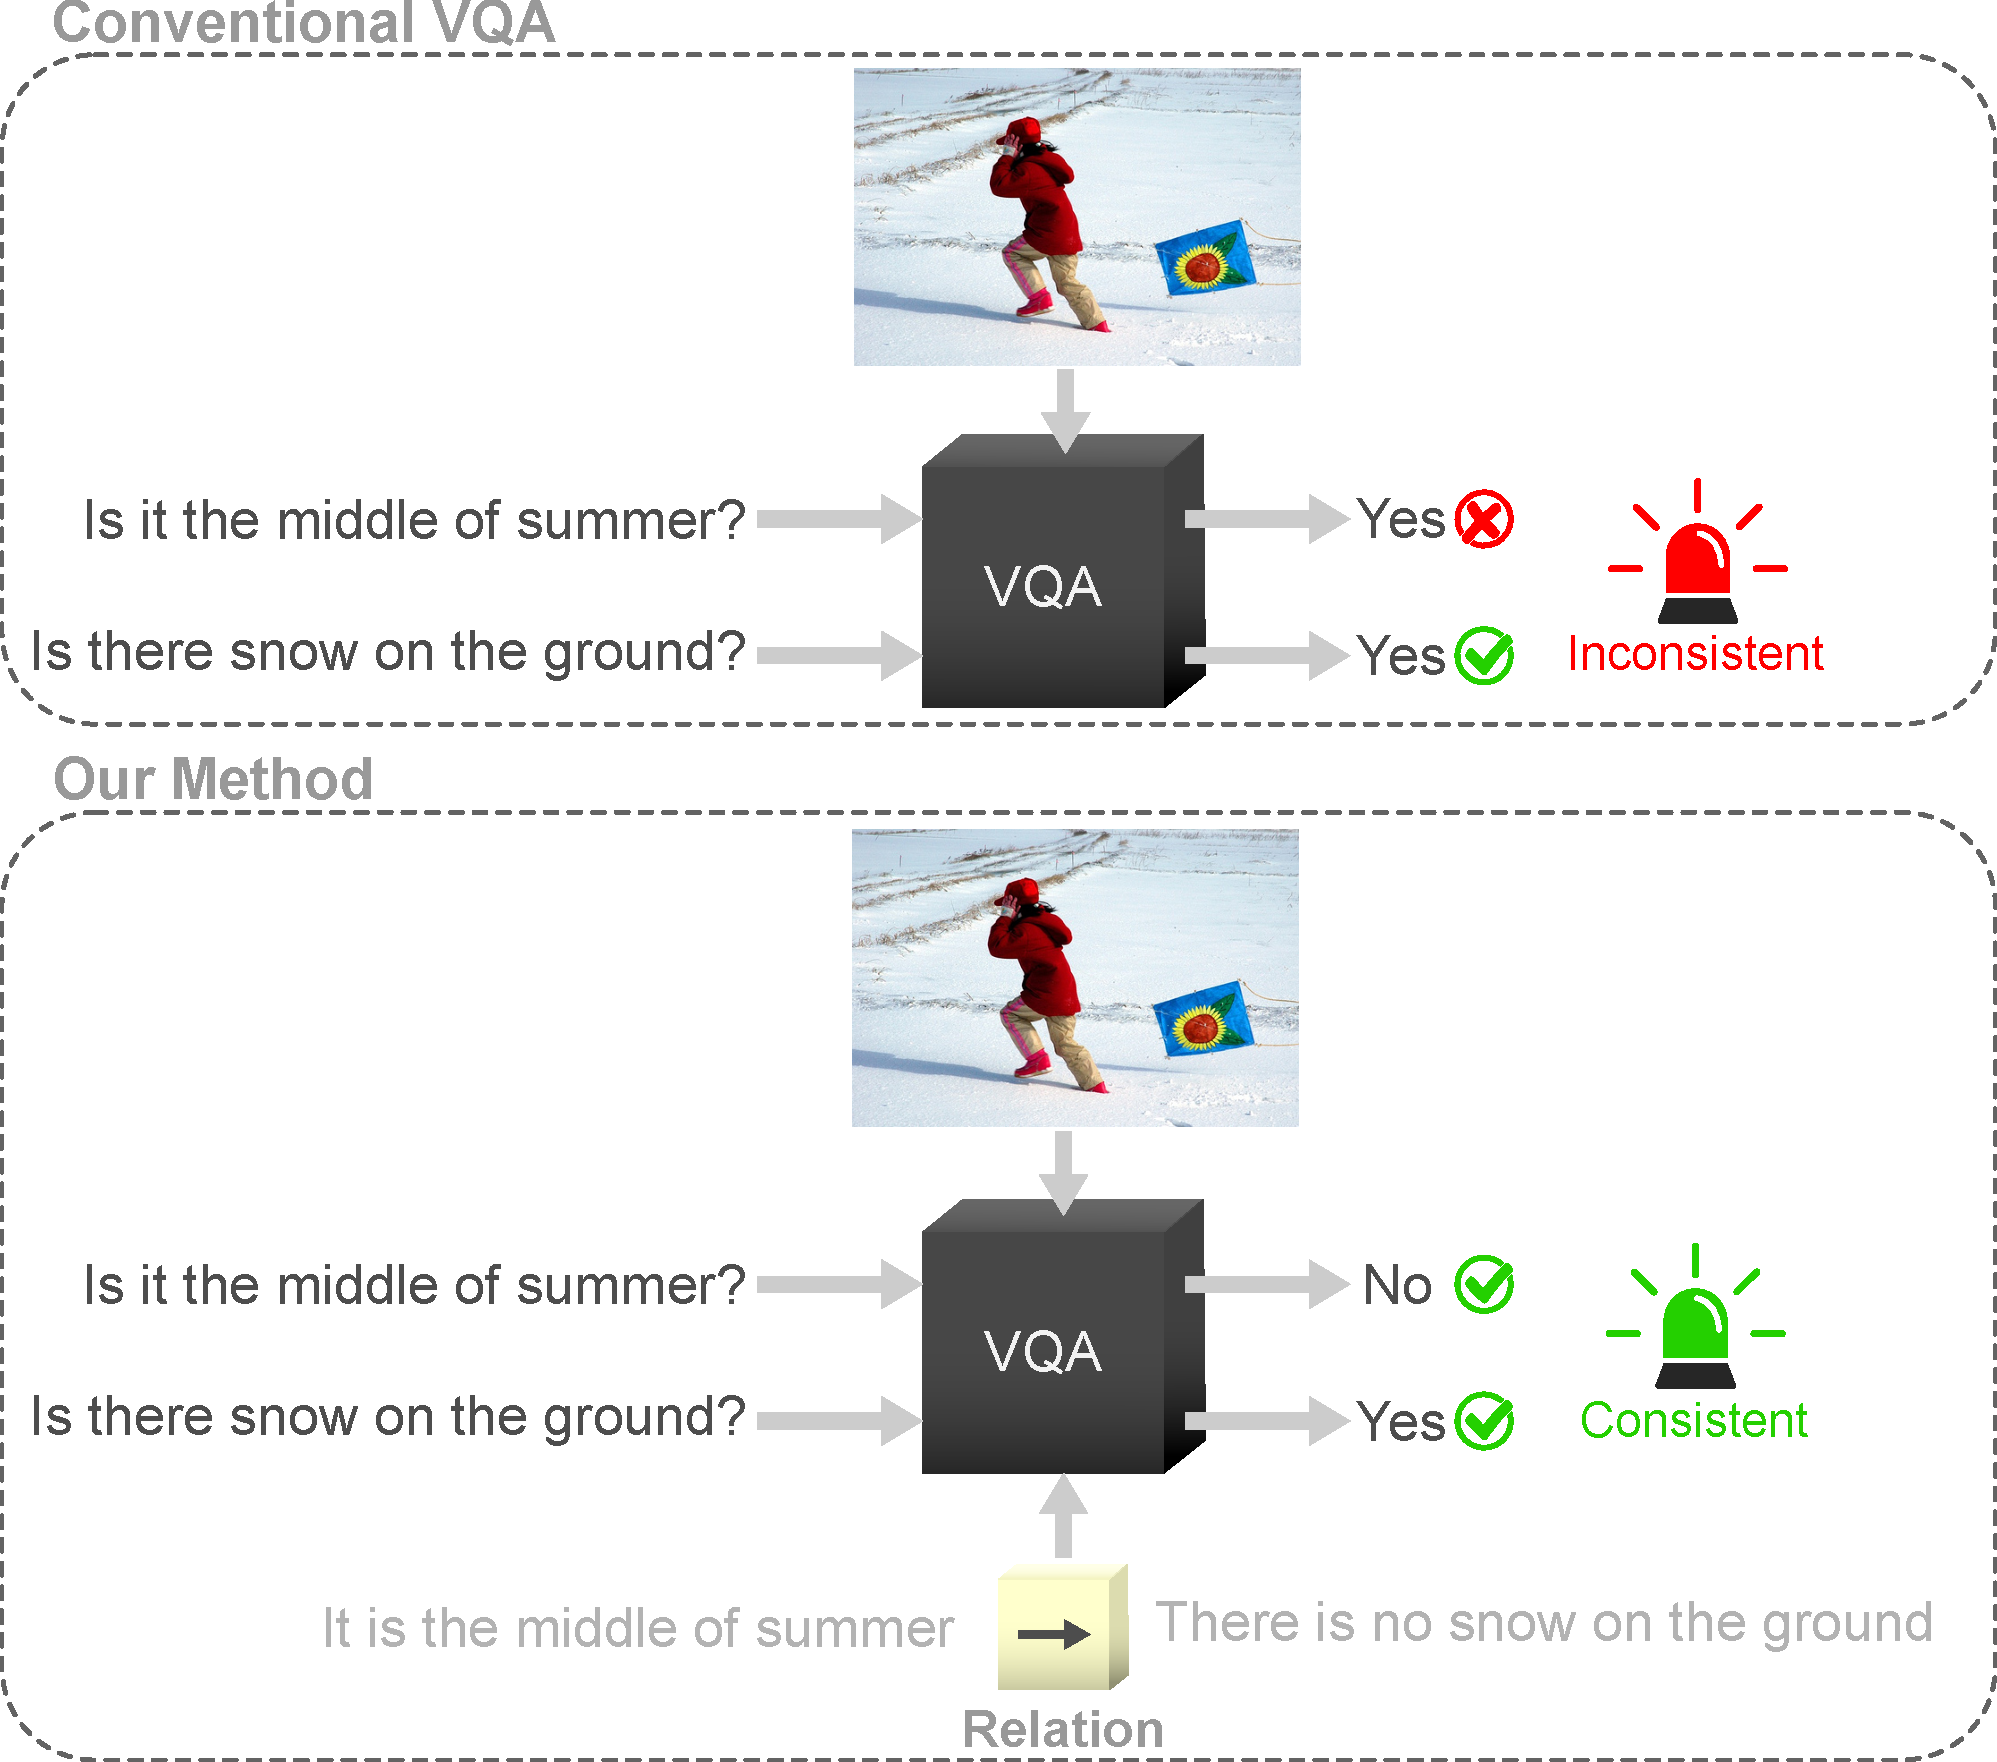
\includegraphics[width=0.6\textwidth]{Figures/Part2_Consist/02_logic/image_intro.pdf}
\caption{\textbf{Top:} Conventional VQA models tend to produce inconsistent answers as a consequence of not considering the relations between question and answer pairs. \textbf{Bottom:} Our method learns the logical relation between question and answer pairs to improve consistency.
} 
\label{fig:image_intro}
\end{figure}

We wish to ensure that \gls{vqa} models are consistent in answering questions about images. This implies that if multiple questions are asked about the same image, the model's answers should not contradict themselves. For instance, if one question about the image in \fig~\ref{fig:image_intro} asks ``Is there snow on the ground?", then the answer inferred should be consistent with that of the question ``Is it the middle of summer?" As noted in~\cite{selvaraju2020squinting}, such question pairs involve reasoning and perception, and consequentially lead the authors to define inconsistency when the reasoning and perception questions are answered correctly and incorrectly, respectively. Along this line,~\cite{tascon2022consistency} uses a similar definition of inconsistency to regularize a \gls{vqa} model meant to answer medical diagnosis questions that are hierarchical in nature. What is critical in both cases, however, is that the consistency of the \gls{vqa} model depends explicitly on its answers, as well as the question and true answer. This hinges on the assumption that perception questions are sufficient to answer reasoning questions. Yet, for any question pair, this may not be the case. As such, the current definition of consistency (or inconsistency) has been highly limited and does not truly reflect how \gls{vqa}s should behave. 

To address the need to have self-consistent \gls{vqa} models, we propose a novel training strategy that relies on logical relations. To do so, we re-frame question-answer (QA) pairs as propositions and consider the relational construct between pairs of propositions. This construct allows us to properly categorize pairs of propositions in terms of their logical relations. From this, we introduce a novel loss function that explicitly leverages the logical relations between pairs of questions and answers in order to enforce that \gls{vqa} models be self-consistent. However, datasets typically do not contain relational information about QA pairs, and collecting this would be extremely laborious and difficult. To overcome this, we propose to train a dedicated language model that infers logical relations between propositions.
Our experiments show that we can effectively infer logical relations from propositions and use them in our loss function to train \gls{vqa} models that improve state-of-the-art methods via consistency. We demonstrate this over two different \gls{vqa} datasets, against different consistency methods, and with different \gls{vqa} model architectures.

\subsection{Previous Work}
Since its initial presentation in Antol et al.~\cite{antol2015vqa}, \gls{vqa} has thoroughly advanced. Initial developments focused on multimodal fusion modules, which combine visual and text embeddings~\cite{nam2017dual,cadene2019murel}. From basic concatenation and summation~\cite{antol2015vqa} to more complex fusion mechanisms that benefit from projecting the embeddings to different spaces, numerous approaches have been proposed~\cite{fukui2016multimodal,kim2016hadamard,ben2017mutan}. The addition of attention mechanisms~\cite{kim2018bilinear, nam2017dual,cadene2019murel} and subsequently transformer architectures~\cite{vaswani2017attention} has also contributed to the creation of transformer-based \gls{vlm}, such as LXMERT, which have shown state-of-the-art performances~\cite{tan2019lxmert}. 

More recently, methods have proposed to improve other aspects of \gls{vqa}, including avoiding shortcut learning and biases~\cite{dancette2021beyond,han2021greedy}, improving 3D spatial reasoning~\cite{banerjee2021weakly}, Out-Of-Distribution (OOD) generalization~\cite{cao2021linguistically,teney2020unshuffling}, improving transformer-based vision-language models~\cite{yang2021auto,zhou2021trar}, external knowledge integration~\cite{ding2022mukea,gao2022transform} and model evaluation with visual and/or textual perturbations~\cite{gupta2022swapmix,walmer2022dual}. With the awareness of bias in \gls{vqa} training data, some works have also addressed building better datasets (\eg, VQAv2.0~\cite{goyal2017making}, VQA-CP~\cite{agrawal2018don}, CLEVR~\cite{johnson2017clevr} and GCP~\cite{hudson2019gqa}).

Furthermore, these developments have now given rise to \gls{vqa} methods in specific domains. For instance, the VizWiz challenge~\cite{gurari2018vizwiz,gurari2019vizwiz,chen2022grounding} aims at creating \gls{vqa} models that can help visually impaired persons with routine daily tasks, while there is a growing number of \gls{medvqa} works with direct medicine applications~\cite{nguyen2019overcoming,gupta2021hierarchical,vu2020question,zhan2020medical}. 

\subsubsection{Consistency in VQA} Consistency in \gls{vqa} can be defined as the ability of a model to produce answers that are not contradictory. This is, given a pair of questions about an image, the answers predicted by a \gls{vqa} model should not be contrary (\eg answering ``Yes" to ``Is it the middle of summer?" and ``Winter" to ``What season is it?"). Due to its significance in reasoning, consistency in \gls{vqa} has become a focus of study in recent years~\cite{ribeiro2019red,shah2019cycle,gokhale2020vqa,selvaraju2020squinting,jing2022maintaining}. Some of the first approaches for consistency enhancement focused on creating re-phrasings of questions, either by dataset design or at training time~\cite{shah2019cycle}. Along this line, entailed questions were proposed~\cite{ribeiro2019red,gokhale2020vqa}, such that a question generation module was integrated into a \gls{vqa} model~\cite{ray2019sunny,goel2021iq}, used as a benchmarking method to evaluate consistency~\cite{yuan2021perception} or as a rule-based data-augmentation technique~\cite{ribeiro2019red}. Other approaches tried to shape the embedding space by imposing constraints in the learned representations~\cite{teney2019incorporating} and by imposing similarities between the attention maps of pairs of questions~\cite{selvaraju2020squinting}. Another work~\cite{tascon2022consistency} assumed entailment relations between pairs of questions to regularize training. A more recent approach attempts to improve consistency by using graph neural networks to simulate a dialog in the learning process~\cite{jing2022maintaining}. 

While these approaches show benefits in some cases, they typically only consider that a subset of logical relationships exists between pairs of question-answers or assume that a single relation holds for all QA pairs. Though true in the case of re-phrasings, other question generation approaches cannot guarantee that the produced questions preserve unique relations or that grammatical structure remains valid. Consequently, these methods often rely on metrics that either over or under-estimate consistency by relying on these assumptions. In the present work, we propose a strategy to alleviate these limitations by considering all logical relations between pairs of questions and answers. 

\subsubsection{Entailment Prediction} \glsxtrfull{nli}, or \gls{rte}, is the task of predicting how two input sentences (namely \textit{premise} and \textit{hypothesis}) are related, according to three pre-established categories: entailment, contradiction and neutrality~\cite{maccartney2008modeling}. For example, if the premise is ``A soccer game with multiple males playing" and the hypothesis is ``Some men are playing a sport," then the predicted relation should be an entailment, because the hypothesis logically follows from the premise. Several benchmarking datasets (\eg, SNLI~\cite{young2014image}, MultiNLI~\cite{williams2017broad}, SuperGLUE~\cite{wang2019superglue}, WIKI-FACTCHECK~\cite{sathe2020automated} and ANLI~\cite{nie2019adversarial}) have contributed to the adaption of general-purpose transformer-based models like \gls{bert}~\cite{devlin2018bert}, RoBERTa~\cite{liu2019roberta} and DeBERTa~\cite{he2020deberta} for this task. In this work, we will leverage these recent developments to build a model capable of inferring relations between propositions.
\section{Method}


\label{sec:method}
Given an image $\x \in \mathcal{I}$, a question $\q \in \mathcal{Q}$ about the image and a set $\mathcal{A}=\{a_1,\ldots, a _K\}$ of possible answers to choose from, a \gls{vqa} model is expected to infer the answer $\hat{a} \in \mathcal{A}$ that matches the true answer $a^*$. This can be formulated as, 
\begin{equation}
    \hat{a} = \argmax_{a \in \mathcal{A}} p(a | \x,\q; \bm{\theta}),
    \label{eq:vqa}
\end{equation}
where $\bm{\theta}$ represents the parameters of the \gls{vqa} model.

% In this context, consider the relation between two QA pairs $(\q _i, a_i)$ and $(\q_j, a_j)$ for the same image $\x$ -- for example, the pairs (``Is the horse brown?", ``No") and (``What is the color of the horse?", ``White"). In this case the first pair is a necessary condition for the second one or, equivalently, the second pair is a sufficient condition for the first one.

In this context, we observe that two QA pairs $(\q _i, a_i)$ and~$(\q_j, a_j)$ for the same image~$\x$ can have different kinds of logical relations. In the simplest case, the two pairs may be unrelated, as with the pairs (``Is it nighttime?'', ``Yes'') and (``Is there a bench in the image?'', ``No''). Knowing that one of the pairs is true gives no information about the truth value of the other. 

On the other hand, two pairs may be related by a logical implication, as in the pairs (``Is the horse brown?", ``No") and (``What is the color of the horse?", ``White"). Knowing that the second pair is true implies that the first pair must be true as well. Conversely, if the first pair is false (\emph{the horse is brown}), it implies that the second pair must also be false. In this case, the first pair is a necessary condition for the second one or, equivalently, the second pair is a sufficient condition for the first one. 

Finally, it can be that two QA pairs are related by a double logical implication, as with the pairs (``Is this a vegetarian pizza?'', ``Yes'') and (``Does the pizza have meat on it?'', ``No''). The veracity of the former implies the veracity of the latter, but the veracity of the latter also implies the veracity of the former. In this case, each pair is simultaneously a necessary and sufficient condition for the other pair, and both pairs are then equivalent. 

Note that the logical implication existing between two QA pairs is an intrinsic property of the QA pairs, and does not depend on the correctness of the predictions coming from a \gls{vqa} model. If a \gls{vqa} model considers a sufficient condition true and a necessary condition false, it is incurring an \emph{inconsistency} regardless of the correctness of its predictions.
% When discussing logical implications, we will only care about the truth values of the QA pairs, but not whether the VQA model

Since logical implications are the basis of reasoning, we propose to explicitly use them when training a \gls{vqa} model to reduce its inconsistent predictions.
% If we now consider any potential pair of QAs, then four possible {logical interactions} could be observed: (1) sufficient, (2) necessary, (3) equivalent or (4) unrelated. Since these types of relationships are the basis of reasoning, we propose to explicitly use them when training a VQA model to reduce its inconsistent predictions.
Unfortunately, doing so requires overcoming two important challenges: (1)~a strategy is needed to train \gls{vqa} models with logical relations that leverage consistency in a purposeful manner. Until now, no such approach has been proposed; (2)~\gls{vqa} datasets do not typically contain logical relations between pairs of QA. Acquiring these manually would, however, be both time-consuming and difficult.

We address these challenges in this work by formalizing the idea of consistency and treating QA pairs as logical propositions from which relations can comprehensively be defined. Using this formalism, we first propose a strategy to solve (1) and train a \gls{vqa} model more effectively using logical relations and the consistency they provide~(Sec.~\ref{subsec:loss}). We then show in Sec.~\ref{subsec:relation_prediction} how we infer relations between pairs of propositions, thereby allowing standard \gls{vqa} datasets to be augmented with logical relations.

%%----------------------------$$

%\begin{figure*}[!t]
%\centering
%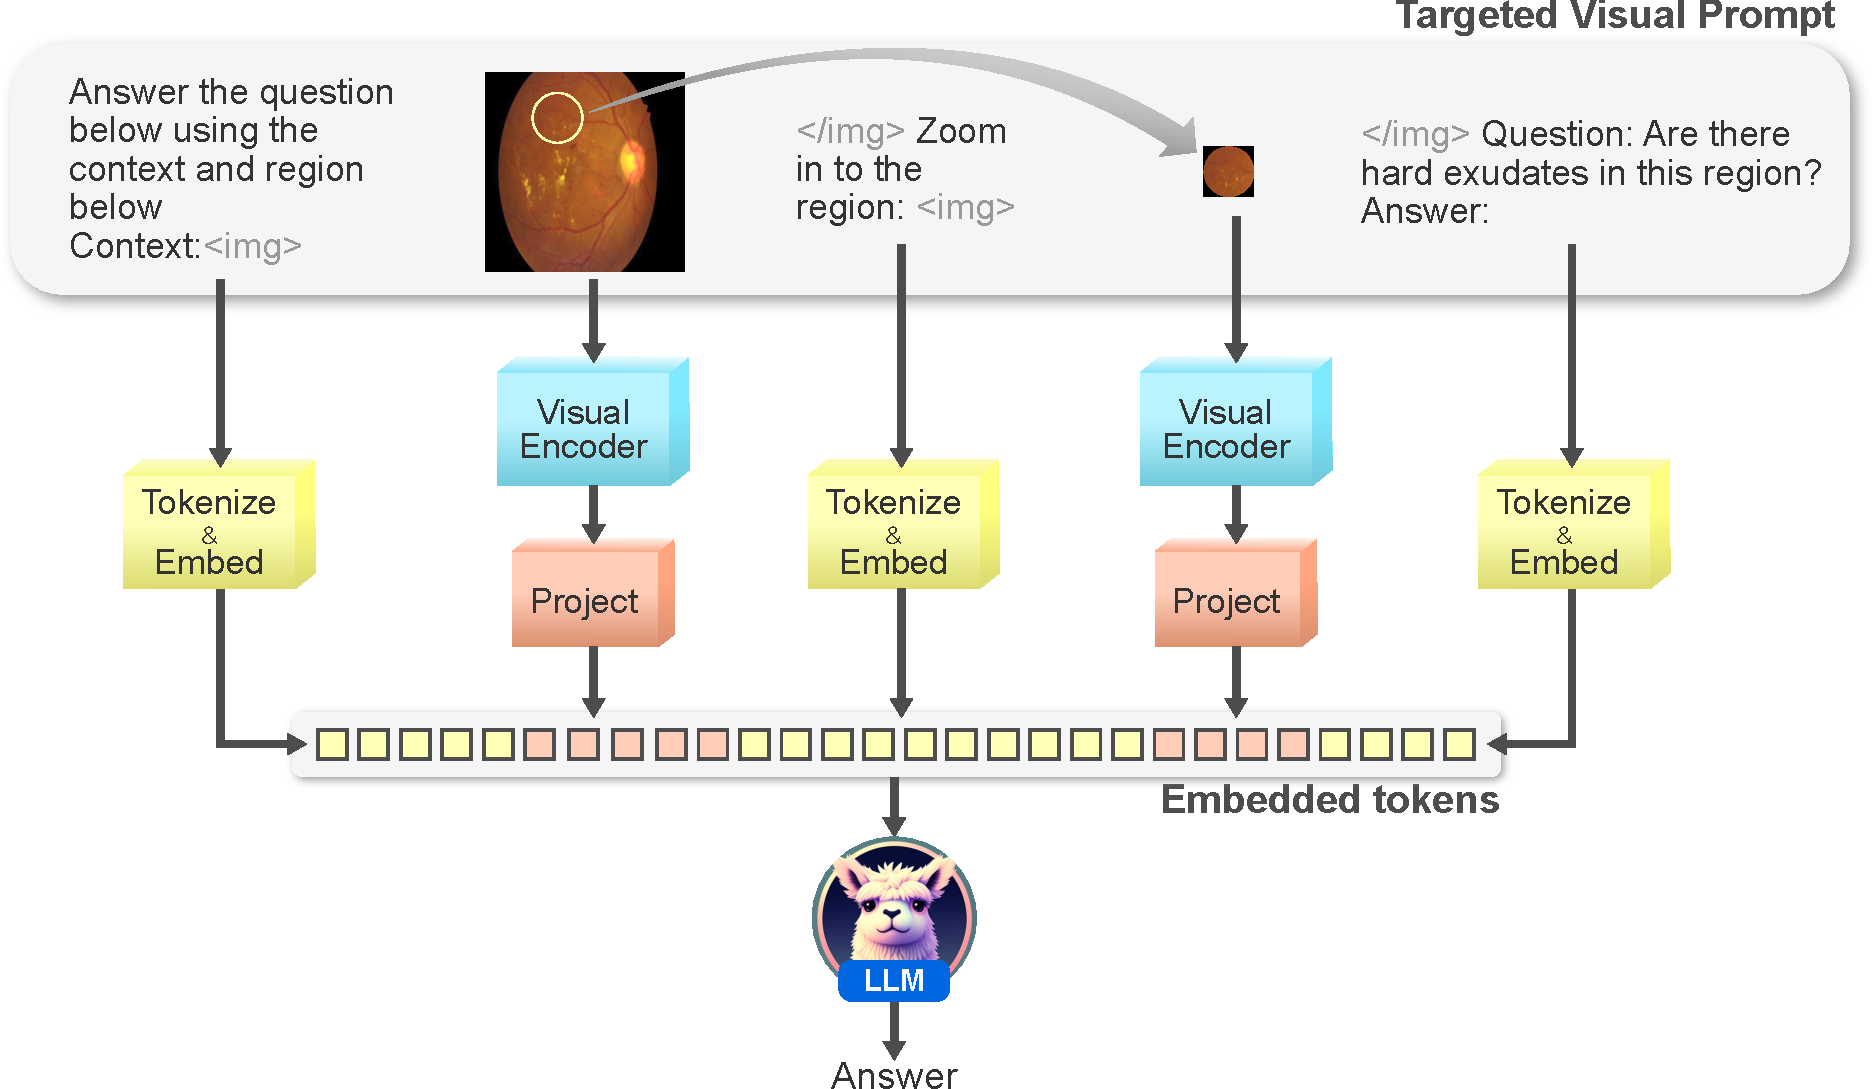
\includegraphics[width=0.85\textwidth]{images/method.pdf}
%\caption{Overview of our method. The VQA model receives a batch of images and questions that has been sampled so that related questions are consecutive. The scores provided by the model are used to compute a common VQA loss $\ell_{\textrm{VQA}}$, as well as the proposed consistency loss $\ell_{\textrm{cons}}$. For the latter, the logical implications between the pairs of question-answers are considered so as to avoid inconsistent cases.}
%\label{fig:method}
%\end{figure*}


\subsection{Consistency Formulation}
\label{subsec:consistency_framework}

We begin by observing that QA pairs~$(\q, a)$ can be considered and treated as logical propositions.
For instance, the QA (``Is it winter?", ``Yes") can be converted to ``It is winter," which is a logical proposition that can be evaluated as \emph{true} or \emph{false} (\ie,~its \emph{truth value}). Doing so allows us to use a broad definition of consistency, namely one that establishes that two propositions are inconsistent if both cannot be true at the same time~\cite{bradley1979possible}. In the context of this work, we assume the truth value of a proposition~$(\q, a)$ is determined by an agent (either a human annotator or the \gls{vqa} model) after observing the information contained in an image~$\x$. 

Let $\mathcal{D} = \mathcal{I}\times \mathcal{Q} \times \mathcal{A}$ be a \gls{vqa} dataset that contains triplets $(\x^{(n)}, \q_i^{(n)}, a_i^{(n)})$, where $\x^{(n)}$ is the $n$-th image and $(\q_i^{(n)}, a_i^{(n)})$ is the $i$-th question-answer pair about $\x^{(n)}$. In the following, we omit the index~$n$ for succinctness. For a given image $\x$, we can consider a pair of related question-answers as $(\q_i, a_i)$ and $(\q_j, a_j)$ as a pair of propositions. 
Following propositional logic notation, if both propositions are related in such a way that $(\q_i, a_i)$~is a sufficient condition for the necessary condition $(\q_j, a_j)$, we write that $(\q_i, a_i)\rightarrow (\q_j, a_j)$. For convenience, this arrow notation can be adapted to indicate different orderings between the necessary and sufficient conditions:
\begin{itemize}
    \item $(\q_i, a_i) \leftarrow (\q_j, a_j)$ if the proposition $(\q_i,a_i)$ is a necessary condition for $(\q_j,a_j)$. %: \ie, the falsity of $(\q_i,a_i)$ guarantees the falsity of $(\q_j,a_j)$.
    % \item $(\q_i, a_i) \rightarrow (\q_j, a_j)$ if the proposition $(\q_i,a_i)$ is a sufficient condition for $(\q_j,a_j)$: \ie, the truth of $(\q_i,a_i)$ guarantees the truth of $(\q_j,a_j)$. %\PMN{I'm a bit confused. Isn't $(\q_i, a_i) \rightarrow (\q_j, a_j)$ the same as $(\q_j, a_j) \leftarrow (\q_i, a_i)$? Why do we need two different arrows? Is the order of the pair of propositions important?} %\STM{It is not strictly necessary but it serves a function in the definition and using it simplifies the training so that we don't have to deal with the order of the pairs}
    \item $(\q_i, a_i) \leftrightarrow (\q_j, a_j)$ if the propositions $(\q_i,a_i)$ and $(\q_j,a_j)$ are equivalent, \ie, both are simultaneously necessary and sufficient. Note that this is just notational convenience for the double implication $(\q_i, a_i) \rightarrow (\q_j, a_j) \wedge (\q_j, a_j) \rightarrow (\q_i, a_i)$, and in the following derivations the double arrow will be always considered as two independent arrows.
    \item Finally, we will write $(\q_i, a_i) - (\q_j, a_j)$ if the propositions $(\q_i,a_i)$ and $(\q_j,a_j)$ are not related.
\end{itemize}

If a \gls{vqa} model is asked questions $\q_i$ and $\q_j$ about an image $\x$ and there exists a relation $(\q_i, a_i) \rightarrow (\q_j, a_j)$, the answers of the model will be inconsistent whenever it provides answers $\hat{a}_i = a_i$ and $\hat{a}_j \neq a_j$ (\ie, the model evaluates the first proposition as true and the second proposition as false). More generally, for a pair of necessary and sufficient conditions, the agent will be inconsistent if it evaluates the necessary condition as false and the sufficient condition as true~\cite{bradley1979possible}.
In what follows, we exploit these ideas to quantify model inconsistencies in our experiments and to develop a new loss function that encourages logically consistent \gls{vqa} models.

%%----------------------------$$
%%----------------------------$$

\subsection{Logical Implication Consistency Loss}
\label{subsec:loss}

% Additionally, given that VQAs produce a probability distribution over~$\mathcal{A}$, we can consider a probabilistic evaluation of propositions as
% \begin{equation}
%     e((\q, a), \x) = p(a\mid \x, \q, \theta),
% \end{equation}
% which, instead of the truth value of the proposition, produces the 

%  We propose a consistency loss to improve the reasoning quality of the answers provided by a VQA model. Using the consistency framework described in \ref{subsec:consistency_framework} and the annotations about relations, 


The core aim of our method is to encourage the \gls{vqa} model to avoid inconsistent answers. When training, assume that the model receives an image~$\x$ from~$\mathcal{D}$ and two associated propositions~$(\q_1, a_1)$ and~$(\q_2, a_2)$ that are related by a logical implication~$(\q_1, a_1) \rightarrow (\q_2, a_2)$. We define,
\begin{equation}
    \pi_i=\pi \left((\q_i, a_i), \x \right) = p(a_i\mid \x, \q_i; \bm{\theta}),
\end{equation}
as the probability assigned by the \gls{vqa} model that the proposition~$(\q, a)$ is true for the image~$\x$. The model has a high probability of incurring an inconsistency if it simultaneously gives a high probability~$\pi_1$ to the sufficient condition and a low probability~$\pi_2$ to the necessary condition.

We thus define our consistency loss as a function,
\begin{equation}
    \ell_\textrm{cons}(\x, (\q_1, a_1), (\q_2, a_2)) = - (1-\pi_2) \log(1-\pi_1)  - \pi_1 \log(\pi_2),
\end{equation}
that takes an image and a pair of sufficient and necessary propositions, and penalizes predictions with a high probability of inconsistency. As illustrated in \fig~\ref{fig:loss}, $\ell_\textrm{cons}$~is designed to produce maximum penalties when $\pi_1=1$ and~$\pi_2<1$ (\ie,~when the sufficient condition is absolutely certain but the necessary condition is not), and when $\pi_2=0$ and~$\pi_1>0$ (\ie,~when the necessary condition can never be true but the sufficient condition can be true). At the same time, $\ell_\textrm{cons}$ produces minimum penalties when either $\pi_1=0$ or~$\pi_2=1$, as no inconsistency is possible when the sufficient condition is false or when the necessary condition is true. Interestingly, despite its resemblance, $\ell_\textrm{cons}$ is not a cross-entropy, as it is not an expectation over a probability distribution.

% \begin{figure}
%     \centering
%     \includegraphics[width=0.9\linewidth]{images/loss_3d.png}
%     \caption{Caption}
%     \label{fig:loss_3d}
% \end{figure}

\begin{figure}
    \centering
    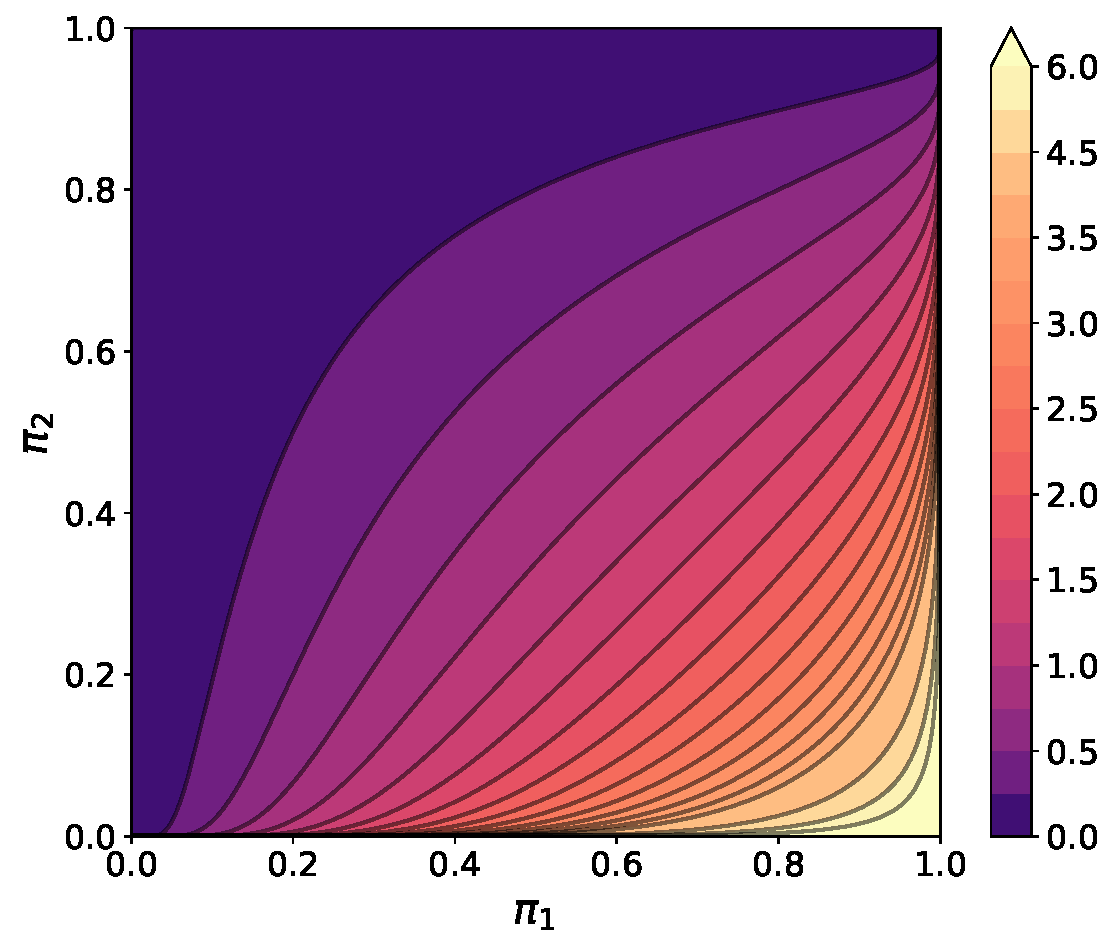
\includegraphics[width=0.5\linewidth]{Figures/Part2_Consist/02_logic/contour.pdf}
    \caption{Consistency loss~$\ell_\textrm{cons}$ as a function of the estimated probabilities for the sufficient,~$\pi_1$, and necessary,~$\pi_2$, conditions. Note that the loss diverges to~$\infty$ when $\pi_1=1, \pi_2<1$ and when~$\pi_1>0, \pi_2=0$.}
    \label{fig:loss}
\end{figure}

% Since the answers that make a pair of question-answers inconsistent depend on the relation between the pair, the value of our consistency term depends on the relation. Given a pair of questions $(\q_i, \q_j)$ about an image $\x$, with ground truth answers $(a_i, a_j)$ and model answers  $(\tilde{a}_i, \tilde{a}_j)$. Depending on the relation $r \in \{\rightarrow, \leftarrow, \leftrightarrow \}$ between $prop(\q_i, a_i)$ and $prop(\q_j, a_j)$, we define the probability terms $w$, $z$, $w^*$ and $z^*$ as shown in \ref{tab:w_z}. This terms represent the probabilities that the model gives inconsistent answers \ie the probability that a relation is violated by having a false necessary condition. For $r= \,\, \leftrightarrow$, we use $w^*$ and $z^*$ to decompose the equivalence into the combination of a necessary condition and a sufficient condition. \PMN{I do not understand these probabilities and the corresponding table. Are these the probabilities predicted by the model?} \STM{They are the probabilities of having inconsistent answers, depending on the relation. They are predicted by the model}
% \begin{table}[!t]
%   \centering
%   \begin{tabular}{@{}ccccc@{}}
%     \toprule
%     $r$ & $w$ & $z$ & $w^*$ & $z^*$  \\
%     \midrule
%     $\rightarrow$ & $p(\tilde{a}_i = a_i)$ & $p(\tilde{a}_j \neq a_j)$ & 0 & 0 \\
%     $\leftarrow$ & $p(\tilde{a}_i \neq a_i)$ & $p(\tilde{a}_j = a_j)$ & 0 & 0\\
%     $\leftrightarrow$ & $p(\tilde{a}_i = a_i)$ & $p(\tilde{a}_j \neq a_j)$ &$p(\tilde{a}_i \neq a_i)$ & $p(\tilde{a}_j = a_j)$ \\
%     \bottomrule
%   \end{tabular}
%   \caption{Probabilities of having inconsistent answers, depending on the relation between the propositions implied by the QA pairs.}
%   \label{tab:w_z}
% \end{table}

% We compute the consistency loss as shown in \ref{eq:consistency_loss}. \STM{Add justification for using this function as opposed to any other function} The intuition behind the choice of this function is the following: Since the terms $w$ and $z$ measure the probability of having inconsistent answers, we want a function that returns high values when both of these probabilities are close to one, and low values otherwise. 

% \begin{equation}
% \begin{split}
%     \ell_{\textrm{cons}}(w, z) =  -w \log (1- z) - z \log(1-w) \\ -w^* \log (1- z^*) - z^* \log(1-w^*)
%     \label{eq:consistency_loss}
% \end{split}
% \end{equation}

Our final loss is then a linear combination of the consistency loss and the cross-entropy loss $\ell_{\textrm{VQA}}$ typically used to train \gls{vqa} models. Training with this loss then optimizes, 
\begin{equation}
    \min_\theta \mathbb{E}_{\mathcal{D}}[\ell_{\textrm{VQA}}] +
    \lambda\mathbb{E}_{\substack{((\x_i, \q_i, a_i), (\x_j, \q_j, a_j))\sim\mathcal{D}^2 \\ \x_i=\x_j, (\q_i, a_i)\rightarrow (\q_j, a_j)}}[\ell_{\textrm{cons}}],
\end{equation}
where the first expectation is taken over the elements of the training set~$\mathcal{D}$ and the second expectation is taken over all pairs of necessary and sufficient propositions from~$\mathcal{D}$ defined for the same image.
In practice, we follow the sampling procedure described in~\cite{selvaraju2020squinting,tascon2022consistency}, where mini-batches contain pairs of related questions. The hyperparameter~$\lambda$ controls the relative strength between the \gls{vqa} loss and the consistency term. %\STM{Maybe in this sub-section some reviewer can wonder how we deal with equivalences (double implications)}
% \PMN{It would be a good idea either add the formula or explain what kind of loss it is (cross-entropy?)} \STM{Done}, 
% so as to optimize the performance while avoiding inconsistent answers. The total loss for training a VQA model is given by \ref{eq:total_loss}, where the hyperparameter $\lambda$ is used to adjust the relative weight of the consistency term $\ell_{\textrm{cons}}$. Our method is depicted in \ref{fig:method}.
% \begin{equation}
%     \ell_{\textrm{total}} = \ell_{\textrm{VQA}}+\lambda\ell_{\textrm{cons}}
%     \label{eq:total_loss}
% \end{equation}

%%----------------------------$$
%%----------------------------$$

\subsection{Inferring Implications}
\label{subsec:relation_prediction}
By and large, \gls{vqa} datasets do not include annotations with logical relations between question-answers pairs, which makes training a \gls{vqa} with $\ell_{\textrm{cons}}$ infeasible. To overcome this, we propose to train a language model to predict logical implications directly and use these predictions instead. We achieve this in two phases illustrated in \fig~\ref{fig:relation_prediction} and refer to our approach as the Logical-Implication model (LI-MOD).

\begin{figure}[!t]
\centering
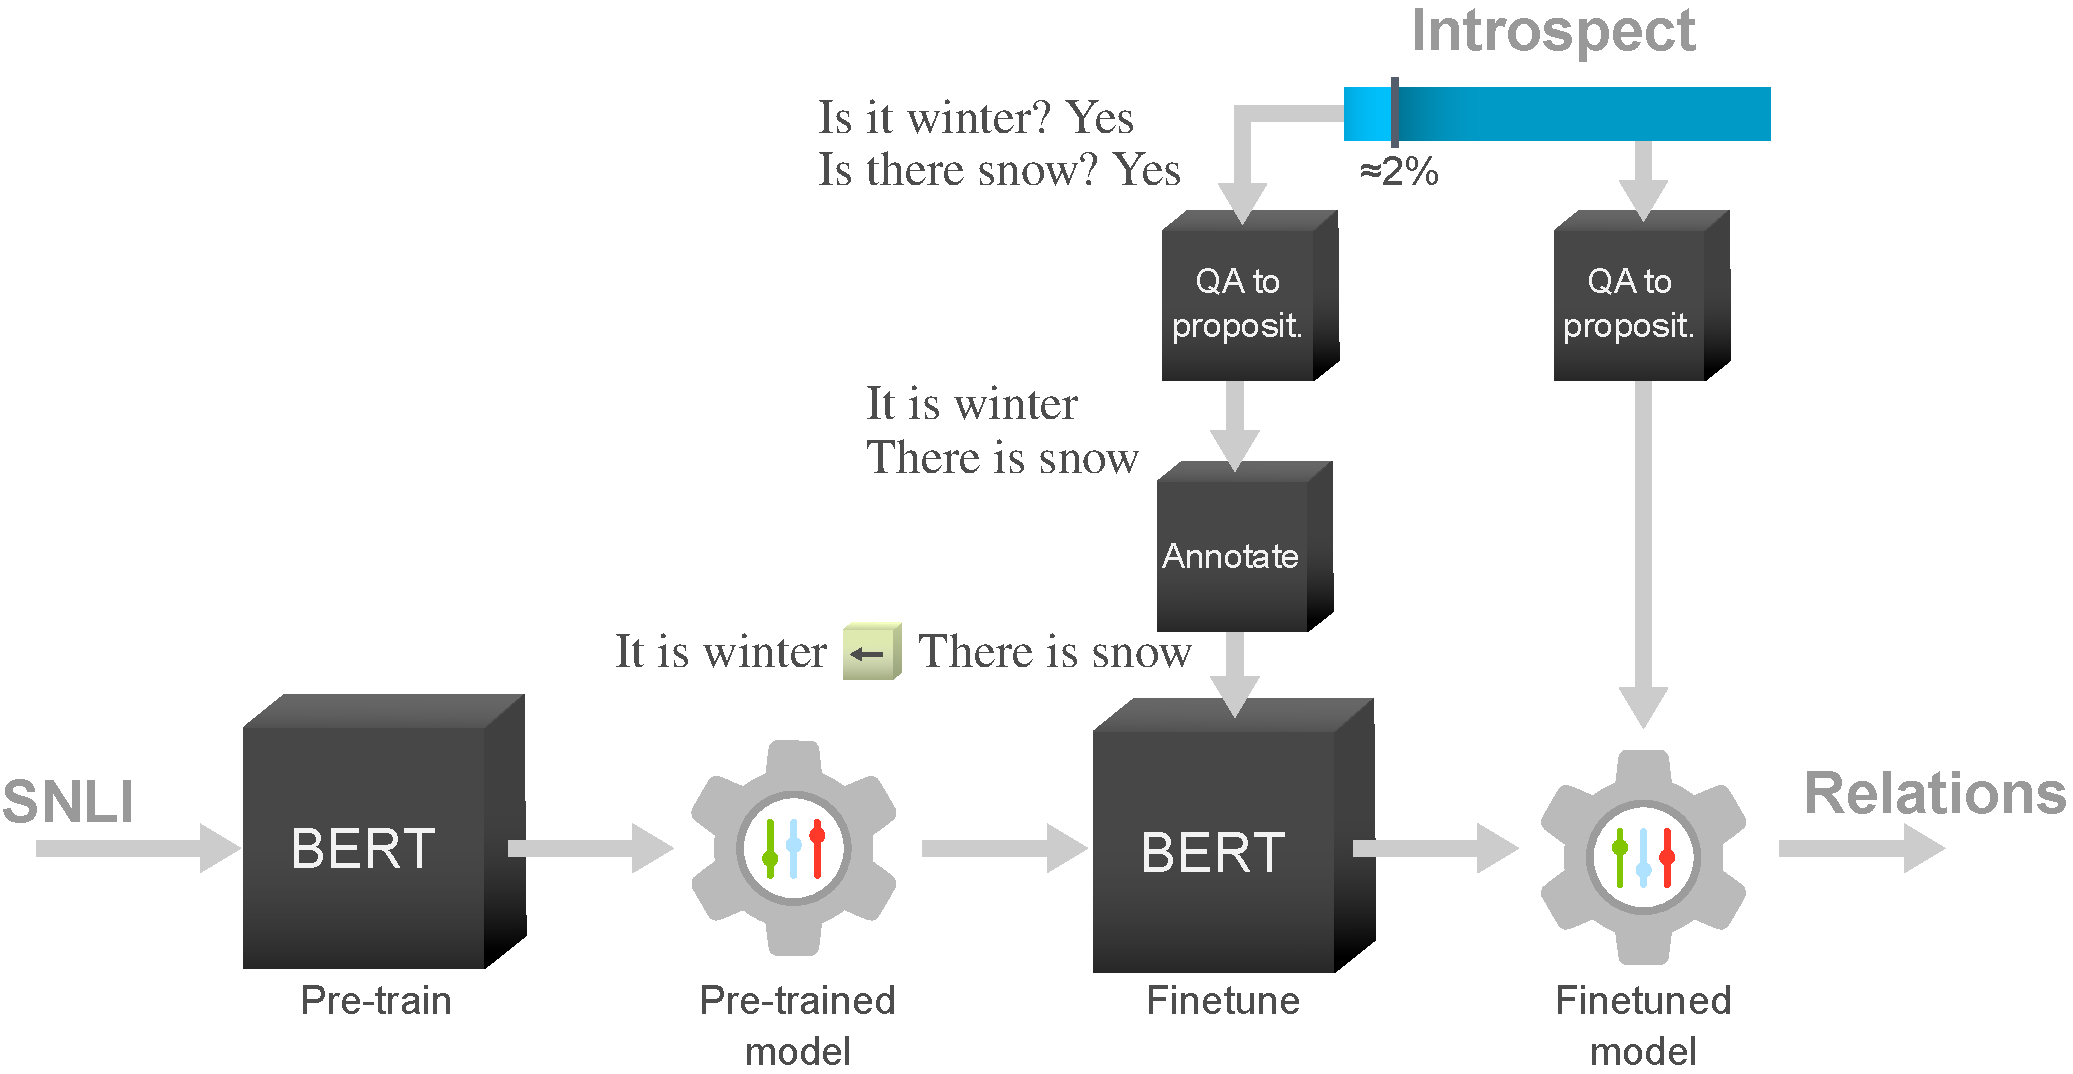
\includegraphics[width=0.7\textwidth]{Figures/Part2_Consist/02_logic/bert_relations.pdf}
    \caption{LI-MOD: Approach to predict logical relations between pairs of propositions. A BERT-based NLP model is first pre-trained on the SNLI dataset~\cite{young2014image} to solve a Natural Language Inference task and subsequently fine-tuned with annotated pairs from a subset of Introspect dataset~\cite{selvaraju2020squinting}. The resulting model is used to predict the relations of the remaining part of the dataset.}
\label{fig:relation_prediction}
\end{figure}

First, we pre-train \gls{bert}~\cite{devlin2018bert} on the task of Natural Language Inference using the SNLI dataset~\cite{young2014image}, which consists of pairs of sentences with annotations of entailment, contradiction or neutrality. In this task, given two sentences, a language model must predict one of the mentioned categories. While these categories do not exactly match the logical implication relevant to our objective, they can be derived from the entailment category. To this end, given two propositions $(\q_i,a_i)$ and $(\q_j,a_j)$, we evaluate them using the finetuned \gls{nli} model in the order $(\q_i,a_i),(\q_j,a_j)$, and then repeat the evaluation by inverting the order, to evaluate possible equivalences or inverted relations. If the relation is predicted as neutral in both passes, the pair is considered to be unrelated.

Then, we finetune the \gls{nli} model on a sub-set of annotated pairs from the \gls{vqa} dataset Introspect~\cite{selvaraju2020squinting}. In practice, we use a subset of binary QA pairs that were manually annotated with logical implications. Even though the relation need not be limited to binary questions (\ie, yes/no questions), we chose to do so because the relation annotation is simpler than for open-ended questions. Since BERT expects sentences and not QA pairs, these were first converted into propositions using Parts Of Speech (POS) tagging~\cite{petrov2011universal} and simple rules that apply to binary questions (\eg,~to convert ``Is it winter?," ``Yes" we invert the first two words of the question and remove the question mark). 
%The QA to proposition conversion is followed by the annotation process, for which we built a simple interface that shows pairs and the possible relations to the user so that the adequate relation can be chosen. 
After finetuning the model, the relations were predicted for the remaining part of the dataset. Further implementation details on this are given in~\ref{subsec:imp_details}.

\section{Experiments and Results}
\label{sec:experiments}

We evaluate our proposed consistency loss function on different datasets and using a variety of \gls{vqa} models.

\subsection{Datasets}
\label{subsec:cons_logic_datasets}

\subsubsection{Introspect~\cite{selvaraju2020squinting} } Contains perception questions (or sub-questions) created by annotators for a subset of reasoning questions (or main questions) of the \gls{vqa} v1.0 and v2.0 datasets~\cite{antol2015vqa,goyal2017making}. It contains 27,441 reasoning questions with 79,905 sub-questions in its training set and 15,448 reasoning questions with 52,573 sub-questions for validation. For images that have the same sub-question repeated multiple times, we remove duplicates in the sub-questions for every image in both the train and validation sets.

\subsubsection{DME Dataset~\cite{tascon2022consistency}} Consists of retinal fundus images for the task of \gls{dme} staging. It contains 9,779 QA pairs for training, 2,380 QA pairs for validation and 1,311 QA pairs for testing. There are three types of questions in the dataset: main, sub, and independent questions. Main questions ask about diagnosis information (\ie the stage of the disease) and sub-questions ask about the presence and location of biomarkers. Sub-questions are further subdivided into grade questions, questions about the whole image, questions about a region of the eye called macula, and questions about random regions in the image. To enable questions about image regions, we follow the procedure described in~\cite{tascon2022consistency}, whereby only the relevant region is shown to the model.


%%%%%%%%%%%%%%%%%%%%%%%%%%%%%%%

\subsection{Baseline Methods and Base Models} We consider 3 different consistency enhancement baseline methods. To ensure fair comparisons, all methods use the same \gls{vqa} base models and only differ in the consistency method used. These consist in:\\

{\setlength{\parindent}{0pt}\textit{- None:} Indicating that no consistency preserving method is used with the \gls{vqa} model. This corresponds to the case where $\lambda=0$.}

{\setlength{\parindent}{0pt}\textit{- SQuINT~\cite{selvaraju2020squinting}:} Optimizes consistency by maximizing the similarity between the attention maps of pairs of questions. As such, it requires a \gls{vqa} model that uses guided attention.}

{\setlength{\parindent}{0pt}\textit{- CP-VQA~\cite{tascon2022consistency}:} Assumes entailment relations and uses a regularizer to improve consistency.}


%(1) The case in which no consistency method is used, which corresponds to the case in which $\lambda=0$ in \ref{eq:total_loss}. So that the comparison is fair, for this baseline we also apply the pair sampling method described in \ref{sec:method} (\ie related pairs are in the same mini-batch). 
%(2) SQuINT~\cite{selvaraju2020squinting}, which is a method that aims at optimizing consistency by maximizing the similarity between the attention maps of pairs of questions. (3) Consistency-preserving VQA (C.P. VQA)~\cite{tascon2022consistency}, which assumes entailment relations and uses a regularizer to improve consistency. 

\subsubsection{VQA Architectures} We show experiments using three \gls{vqa} models depending on the dataset used. For experiments on Introspect, we make use of the \gls{ban} model~\cite{kim2018bilinear}, as its structure with guided attention allows the use of SQuINT. In addition, we evaluate the vision-language architecture LXMERT~\cite{tan2019lxmert} on this dataset to evaluate improvement in state-of-the-art, transformer-based \gls{vqa} models. For experiments on the \gls{dme} dataset, we use the base model described in~\cite{tascon2022consistency}, which we denote by MVQA. 


\subsection{Implementation Details}
\label{subsec:imp_details}
\subsubsection{LI-Model} We first pre-train \gls{bert} on SNLI for 5 epochs until it reaches a maximum accuracy of 84.32\% on that dataset. For this pre-training stage, we initialize \gls{bert} with the \textit{bert-base-uncased} weights and use a batch size of~16. We use a weight decay rate of 0.01 and the AdamW optimizer with a learning rate of $2\cdot10^{-5}$. The same setup was kept to finetune the model on a subset of 2'000 pairs of propositions from Introspect which were manually annotated (distribution of labels being: $\leftarrow 60\%, \leftrightarrow 17\%, - 12\%, \rightarrow  11\%$), and an additional 500 pairs were annotated for validation. Notice that LI-MOD is only necessary for the Introspect dataset since, for the \gls{dme} dataset, the implications annotations are available.

\subsubsection{VQA Models}
For our base models, we use the official and publicly available implementations (\gls{ban}~\cite{jackroos2019}, LXMERT~\cite{tan2019lxmert} and MVQA~\cite{tascon2022consistency}) with default configurations. We re-implemented SQuINT~\cite{selvaraju2020squinting} and used the provided implementation of CP-VQA~\cite{tascon2022consistency}, reporting the best results, which were obtained with $\lambda=0.1, \gamma=0.5$ for \gls{ban} and $\lambda=0.5, \gamma=1$ for MVQA (parameters refer to original implementations). For SQuINT, we set the gain of the attention map similarity term to 0.5 for \gls{ban} and 1.0 for MVQA. For Introspect, we train 5 models with different seeds for each parameter set and for \gls{dme}, we train 10 models with different seeds. To train LXMERT, \gls{ban} and MVQA, we use batch sizes of 32, 64 and 128, respectively. Regarding the \gls{vqa} cross-entropy loss, we follow the original implementations and use soft scores for the answers in LXMERT and categorical answers for \gls{ban} and MVQA.

%%%---------------------------%%%
\subsection{Quantifying Consistency}
%$Given a test set, $\mathcal{T}= \{t_n\}^{=1,\ldots,|\mathcal{T}|}$, where $t_n=(\x, \q, a) $ is a test sample triplet, we evaluate the performance of all models using the strict accuracy of predictions as in ~\cite{selvaraju2020squinting,vu2020question} by computing,
%\begin{equation}
%    acc = \frac{1}{|\mathcal{T}|}\sum_{n=1}^{|\mathcal{T}|} 1_{ \{a^n = \tilde{a}^n \}},
%\end{equation}
%where $\tilde{a}^n = \argmax_{a^* \in \mathcal{A}} p(a^* | \x^n,\q^n; \theta)$ is the produced answer of an evaluated method. \STM{I think we could omit the definition of accuracy here. Most recent CVPR papers on consistency only mention that they use accuracy. This would be easier because LXMERT computes the accuracy slightly differenttly due to the soft scores of the GT answers}

Given a test set~$\mathcal{T}= \{t_n\}_{n=1}^{|\mathcal{T}|}$, where $t_n=(\x, \q, a)$ is a test sample triplet, we wish to measure the level of consistency of a \gls{vqa} model~$p$. To this end, we define the set of implications~$G(\mathcal{T}) \subset \mathcal{T}^2$ as the collection of all pairs of test samples~$((\x_i, \q_i, a_i), (\x_j, \q_j, a_j))$ for which~$(\q_i, a_i) \rightarrow (\q_j, a_j)$ and~$\x_i=\x_j$,
% To do so, we define $G_\leftarrow$, $G_\rightarrow$, $G_\leftrightarrow$, $G_\leftrightarrow$ and $G_{-}$ as sets containing all image-question-answer triplets in $\mathcal{T}$ according to their relation. For instance, $G_\leftarrow$ contains all pairs $((\x, \q_i, a_i), (\x, \q_j, a_j))$ for which $(\q_i, a_i) \leftarrow (\q_j, a_j)$. 
and the set of inconsistencies~$I_p(\mathcal{T})$ produced by the \gls{vqa} model as the subset of~$G(\mathcal{T})$ that contains the pairs for which the model evaluated the sufficient condition as true and the necessary condition as false,
\begin{equation}
    \nonumber
    I_p(\mathcal{T}) = \{ (t_i, t_j)\in G(\mathcal{T})\mid
     e_p((\q_i, a_i), \x) \wedge \neg e_p((\q_j, a_j), \x)\}.
\end{equation}
% We count the inconsistencies produced by a VQA model~$p$ evaluated on~$\mathcal{T}$ as the number of times the model evaluates a sufficient condition as true and a necessary condition as false,
% \begin{equation}
%     I_p(\mathcal{T}) = \sum_{(t_i, t_j)\in G(\mathcal{T})} \mathbbm{1}[e_p((\q_i, a_i), \x) \wedge \neg e_p((\q_j, a_j), \x)].
% \end{equation}
The function~$e_p$ returns the truth value of the proposition~$(\q, a)$ for image~$\x$ evaluated by the \gls{vqa} model~$p$,
\begin{equation}
    e_p((\q, a), \x) = [\hat{a}=a],
\end{equation}
where $\hat{a}$ is the answer of maximum probability following Eq.~\eqref{eq:vqa}. In other words, $e_p$~returns whether the estimated answer for question~$\q$ matches the answer of the proposition~$a$.
Finally, the consistency ratio~$c$ for model~$p$ on the test set~$\mathcal{T}$ is the proportion of implications in~$G(\mathcal{T})$ that did not lead to an inconsistency,
\begin{equation}
    c_p(\mathcal{T}) = 1 - \dfrac{|I_p(\mathcal{T})|}{|G(\mathcal{T})|}.
\end{equation}
% \begin{equation}
%     c() = 1 - \frac{I_{\rightarrow} + I_{\leftarrow} + I_{\leftrightarrow}}{|G_{\leftarrow}| + |G_{\leftarrow}| + 2|G_{\leftrightarrow}|}.
%     \label{eq:consistency_metric}
% \end{equation}


% REsults
\subsection{Results}
\label{sec:cons_logic_results}

%%%---------------------------%%%
%%%---------------------------%%%

\subsubsection{Performance Comparison}
For both datasets, we first compare the performance of our method against the baseline consistency methods in Tables \ref{tab:results_introspect} and \ref{tab:cons_logic_results_dme}. In either case, we see that our method outperforms previous approaches by not only increasing overall prediction accuracy but also by increasing consistency. In Figures \ref{fig:examples_introspect} and \ref{fig:examples_dme}, we show illustrative examples of our approach on the Introspect and \gls{dme} datasets, respectively (see additional examples in Appendix~\ref{appendix:consistency_logic}).

%\begin{table}[!b ]
%  \centering
%  \begin{tabular}{@{}lccc@{}}
%    \toprule
%     Model & Cons. Method & Acc. & Cons. \\
%     \midrule
%     BAN & None & 67.14$\pm$0.10 & 69.45$\pm$0.17 \\
%     BAN & SQuINT~\cite{selvaraju2020squinting} & 67.27$\pm$0.19 & 69.87$\pm$0.45 \\
%     BAN & CP-VQA~\cite{tascon2022consistency} & 67.18$\pm$0.24 & 69.52$\pm$0.45\\
%     BAN & {\bf Ours} ($\lambda=0.01$) & {\bf 67.36$\pm$0.19} & {70.38$\pm$0.39} \\
%    \midrule
%    LXMERT & None & 75.10$\pm$0.10 & 76.24$\pm$0.63 \\
%    LXMERT & Random flip & 69.67$\pm$1.24 & 75.99$\pm$3.91\\
%    LXMERT & Flip first & 73.81$\pm$0.47 & 71.94$\pm$2.82\\
%    LXMERT & Flip second & 65.82$\pm$1.03 & {87.56$\pm$2.51}\\
%    LXMERT & {\bf Ours} & {\bf 75.17$\pm$0.08} & {78.75$\pm$0.21} \\
%    \bottomrule
%  \end{tabular}
%  \caption{Results of different consistency methods on the Introspect dataset using two different VQA models: (top) BAN and (bottom) LXMERT. In the case of LXMERT, we show the impact of randomly flipping the answer of either the first or the second question for pairs detected as inconsistent using the relations from LI-MOD. Similarly, {\it flip first} and {\it flip second} refer to flipping the answer of the first and second question in inconsistent pairs, respectively. \STM{STDs added}}
%  \label{tab:results_introspect}
%\end{table}


\begin{table}[!b ]
  \centering
  \begin{tabular}{@{}llcc@{}}
    \toprule
     Model & Cons. Method & Acc. & Cons. \\
     \midrule
     \multirow{4}{*}{BAN} & None & 67.14$\pm$0.10 & 69.45$\pm$0.17 \\
      & SQuINT~\cite{selvaraju2020squinting} & 67.27$\pm$0.19 & 69.87$\pm$0.45 \\
      & CP-VQA~\cite{tascon2022consistency} & 67.18$\pm$0.24 & 69.52$\pm$0.45\\
      & {\bf Ours} ($\lambda=0.01$) & {\bf 67.36$\pm$0.19} & {70.38$\pm$0.39} \\
    \midrule
    \multirow{5}{*}{LXMERT} & None & 75.10$\pm$0.10 & 76.24$\pm$0.63 \\
     & Random flip & 69.67$\pm$1.24 & 75.99$\pm$3.91\\
     & Flip first & 73.81$\pm$0.47 & 71.94$\pm$2.82\\
     & Flip second & 65.82$\pm$1.03 & {87.56$\pm$2.51}\\
     & {\bf Ours} & {\bf 75.17$\pm$0.08} & {78.75$\pm$0.21} \\
    \bottomrule
  \end{tabular}
  \caption{Results of different consistency methods on the Introspect dataset using two different VQA models: \textbf{Top:} BAN, \textbf{bottom:} LXMERT. In the case of LXMERT, we show the impact of randomly flipping the answer of either the first or the second question for related pairs. Similarly, {\it flip first} and {\it flip second} refer to flipping the answer to the first and second question in inconsistent pairs, respectively.}
  \label{tab:results_introspect}
\end{table}

\begin{table*}[t]
\centering
\begin{tabular}{@{}llcccccr@{}}
\toprule
\multirow{2}{*}{Model} &  \multicolumn{1}{l}{\multirow{2}{*}{Consis. Method}}   & \multicolumn{5}{c}{Accuracy}  & \multicolumn{1}{c}{\multirow{2}{*}{Consistency}} \\ \cline{3-7}
\multicolumn{1}{c}{}         &\multicolumn{1}{c}{}                  & \multicolumn{1}{c}{all} & \multicolumn{1}{l}{grade} & \multicolumn{1}{c}{whole} & \multicolumn{1}{c}{macula} & \multicolumn{1}{c}{region} & \multicolumn{1}{l}{}                             \\ 
\midrule
\multirow{4}{*}{MVQA}     &   \multicolumn{1}{l}{None}          & \multicolumn{1}{c}{81.15$\pm$0.49}   & \multicolumn{1}{c}{78.17$\pm$2.07} & \multicolumn{1}{c}{83.44$\pm$1.87} & \multicolumn{1}{c}{87.25$\pm$1.20}  & \multicolumn{1}{c}{80.38$\pm$2.02}  & \multicolumn{1}{c}{89.95$\pm$3.20}                        \\ 

 &  \multicolumn{1}{l}{SQuINT~\cite{selvaraju2020squinting}}& \multicolumn{1}{c}{80.58$\pm$0.78}   & \multicolumn{1}{c}{77.48$\pm$0.40} & \multicolumn{1}{c}{82.82$\pm$0.74} & \multicolumn{1}{c}{85.34$\pm$0.87}  & \multicolumn{1}{c}{80.02$\pm$1.03}  & \multicolumn{1}{c}{89.39$\pm$2.12}               
\\ 

 &  \multicolumn{1}{l}{CP-VQA~\cite{tascon2022consistency}}& \multicolumn{1}{c}{83.49$\pm$0.99}   & \multicolumn{1}{c}{\textbf{80.69$\pm$1.30}} & \multicolumn{1}{c}{84.96$\pm$1.14} & \multicolumn{1}{c}{87.18$\pm$2.18} & \multicolumn{1}{c}{\textbf{83.16$\pm$1.09}}  & \multicolumn{1}{c}{94.20$\pm$2.15}  
\\ 

 &  
\multicolumn{1}{l}{{\bf Ours} ($\lambda=0.25$)}& \multicolumn{1}{c}{\textbf{83.59$\pm$0.69}}   & \multicolumn{1}{c}{80.15$\pm$0.95} & \multicolumn{1}{c}{\textbf{86.22$\pm$1.67}} & \multicolumn{1}{c}{\textbf{88.18$\pm$1.07}}  & \multicolumn{1}{c}{82.62$\pm$1.02}  & \multicolumn{1}{c}{{95.78$\pm$1.19}}  

\\ \bottomrule
                                                 
\end{tabular}
\caption{Comparison of methods on the DME dataset with common MVQA backbone. Accuracy and consistency are reported for all questions, as well as for different medically relevant sub-question categories: grade, whole, macula and region.
}
\label{tab:cons_logic_results_dme}
\end{table*}
\begin{figure*}[!t]
\centering
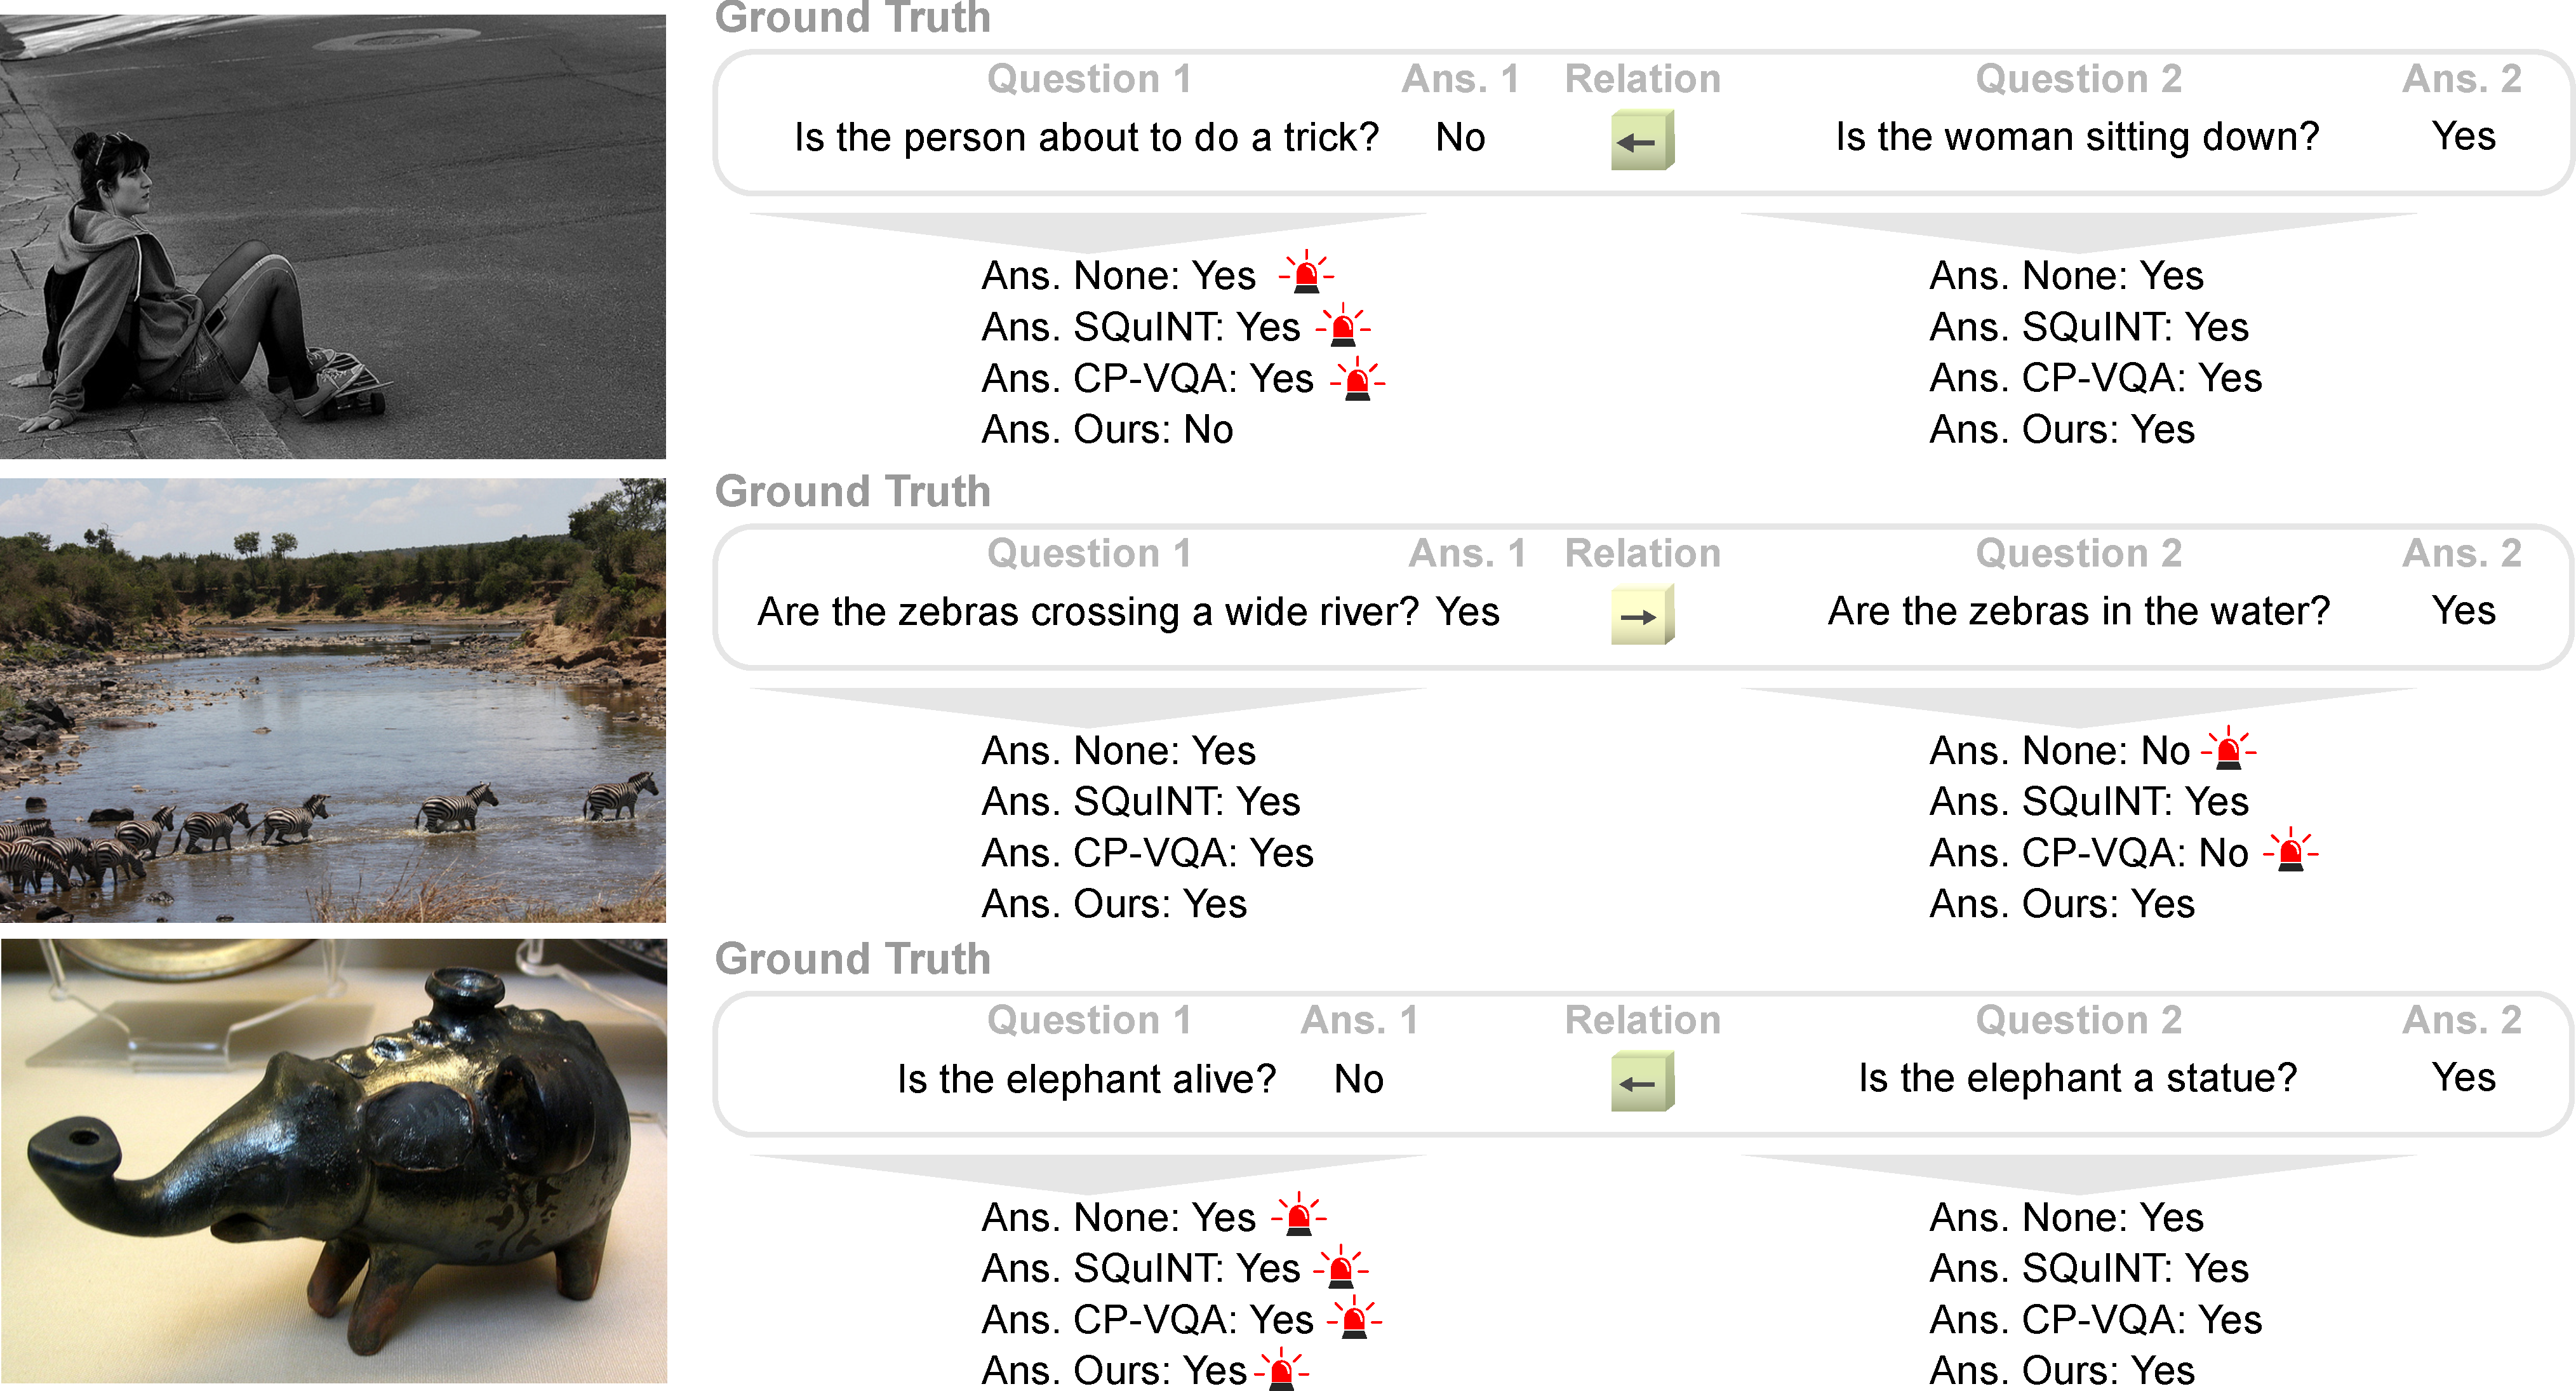
\includegraphics[width=0.95\textwidth]{Figures/Part2_Consist/02_logic/examples_ban.pdf}
\caption{Qualitative examples from the Introspect dataset using BAN as backbone. Red siren symbols indicate inconsistent cases.}
\label{fig:examples_introspect}
\end{figure*}
\begin{figure*}[!t]
\centering
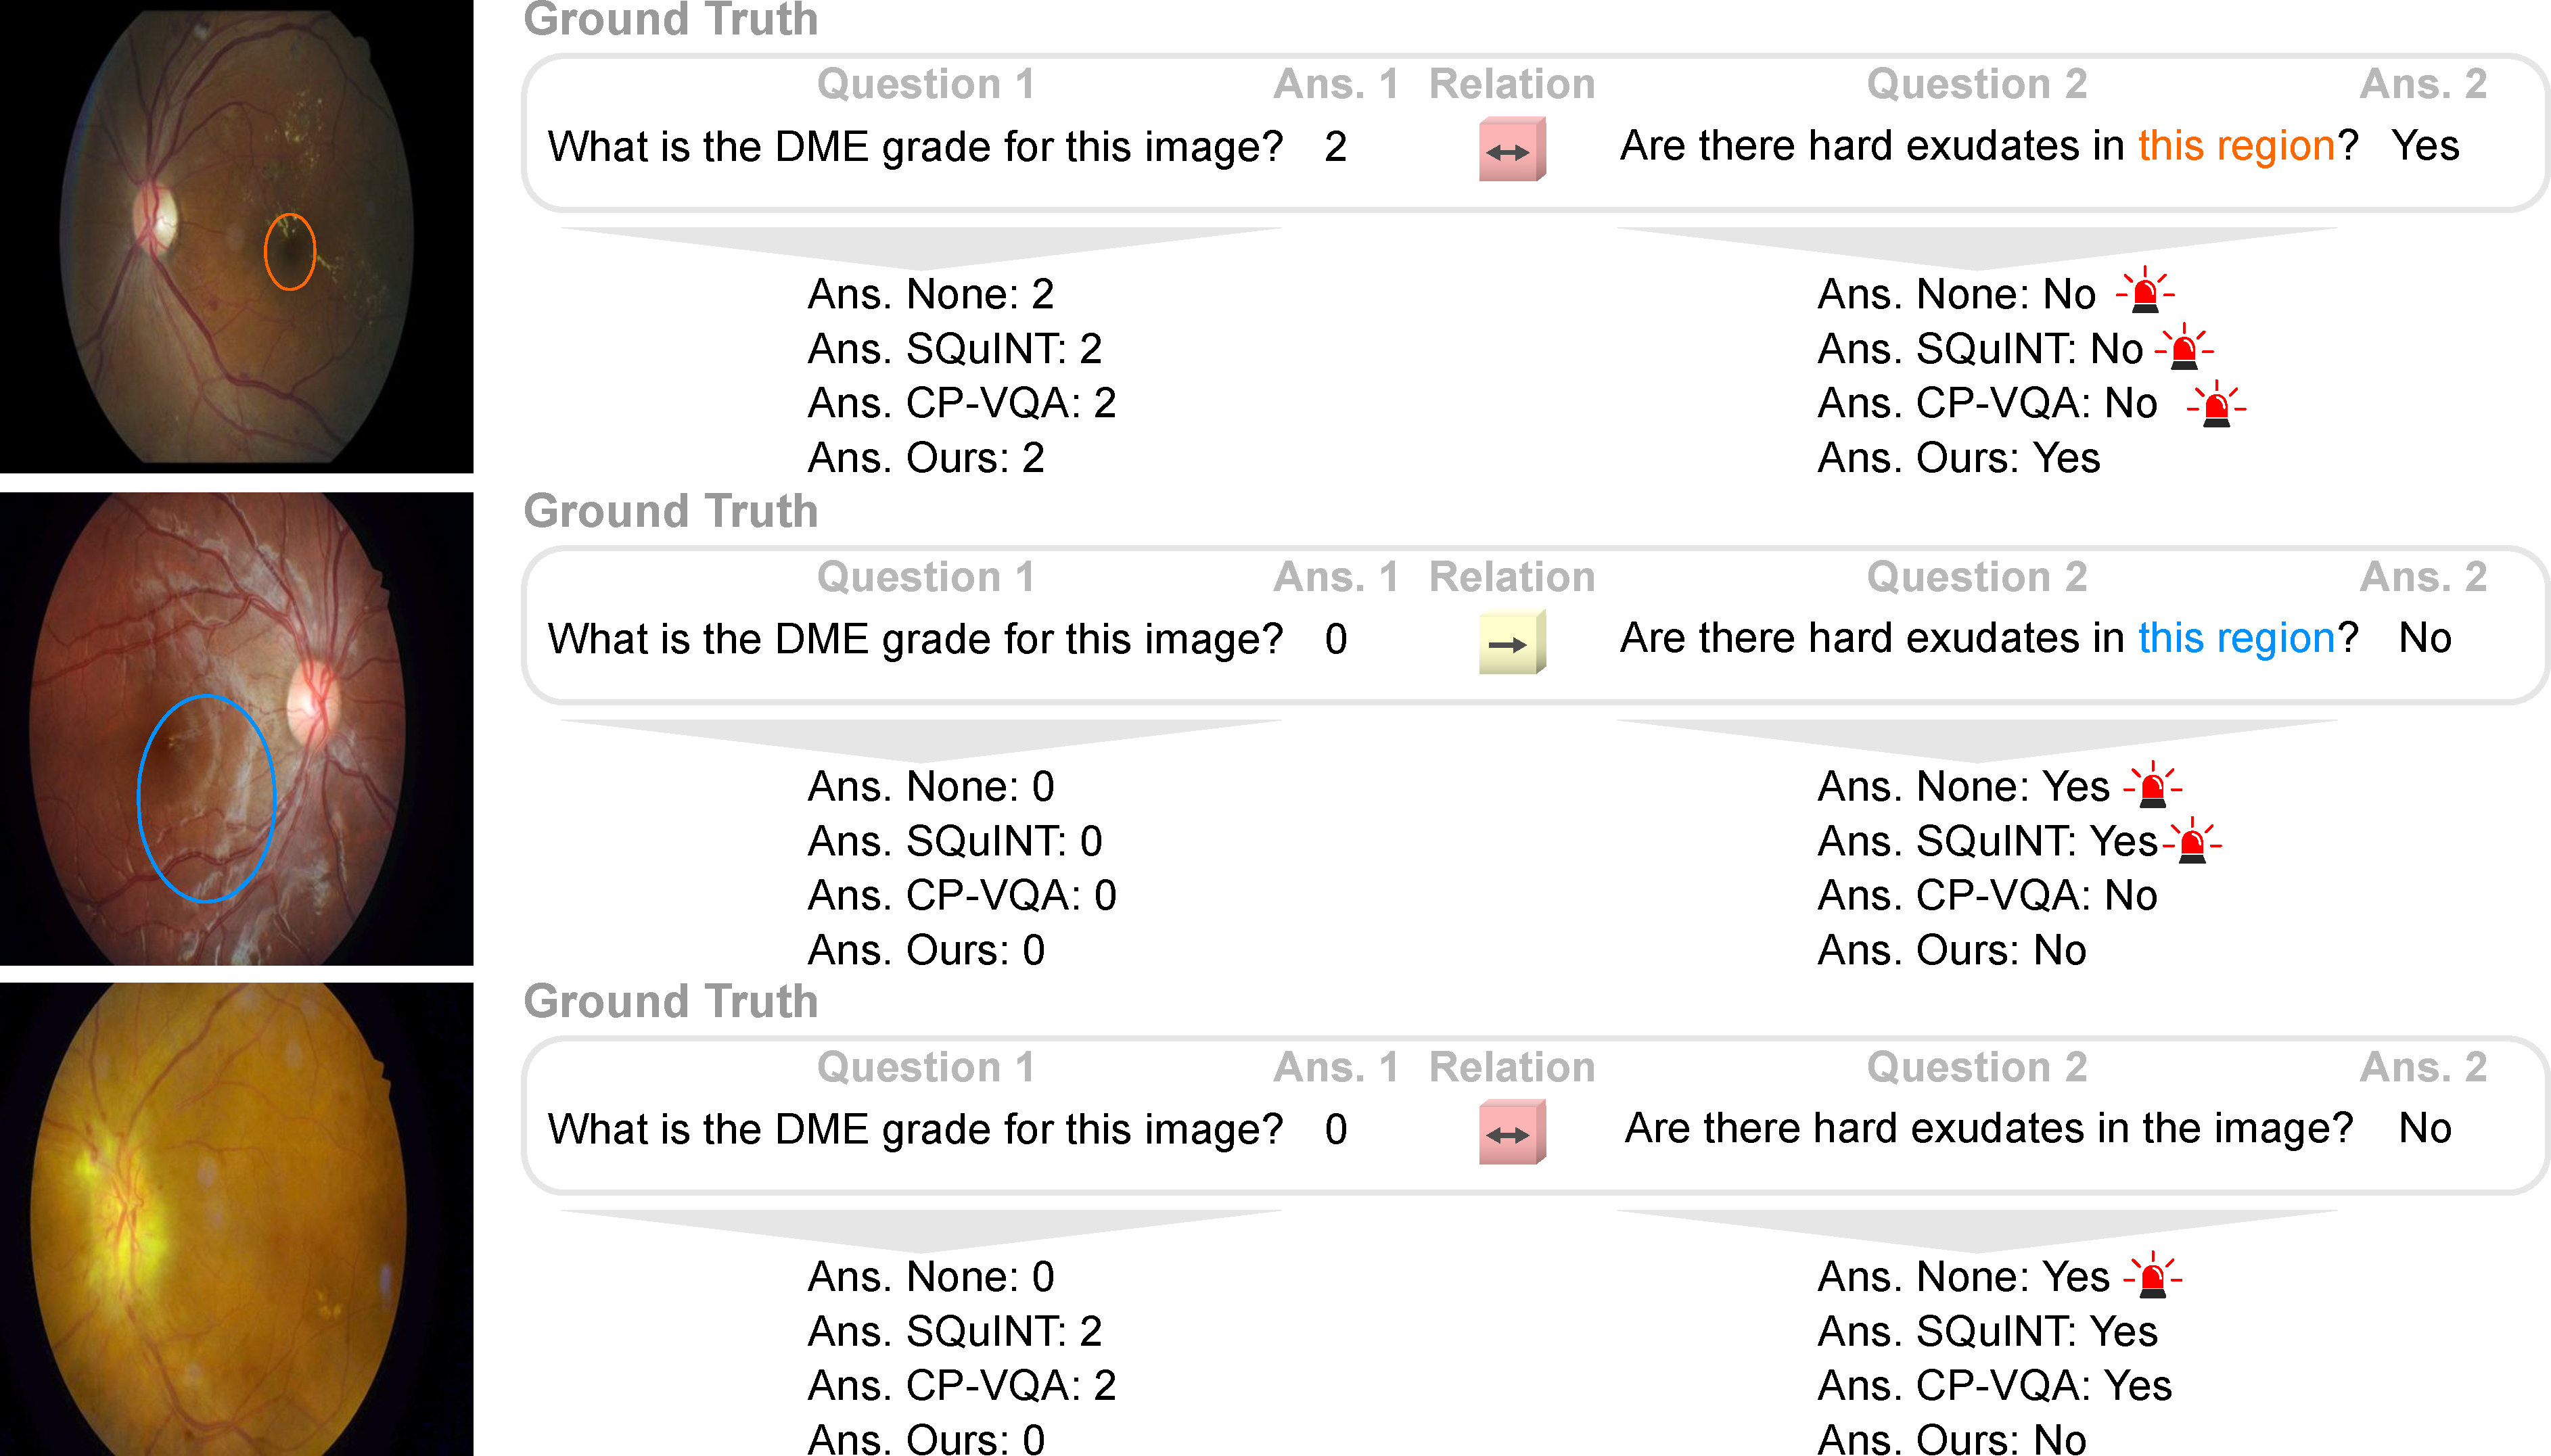
\includegraphics[width=0.90\textwidth]{Figures/Part2_Consist/02_logic/examples_dme.pdf}
\caption{Examples from the DME dataset and comparison of methods. Red siren symbols indicate inconsistent cases. DME is a disease that is staged into grades (0, 1 or 2), which depend on the number of visual pathological features of the retina. \textbf{Top} and \textbf{middle:} Although all methods correctly predict the answer to the first question, some inconsistencies appear when a necessary condition is false. \textbf{Bottom}: Only the None baseline produces an inconsistency. Note that SQuINT and CP-VQA's answers do not produce inconsistent pairs because both questions were answered incorrectly, and those answers (``2" and ``yes") respect all known relations. 
}
\label{fig:examples_dme}
\end{figure*} 

In Table \ref{tab:results_introspect}, we also show the performance of the state-of-the-art LXMERT \gls{vqa} model when combined with our method. In this case, too, we see that our method provides increased performance via consistency improvements. Here we investigate the performance induced when flipping the answers of one of the members of each related pair at test time. Suppose implication labels are present, either by manual annotation or by LI-MOD. In that case, a trivial manner of correcting an inconsistent QA pair of binary answers is to flip or negate one of the answers. This is far simpler than our proposed method as it permits training the \gls{vqa} model with the standard \gls{vqa} loss. Having obtained the answers from the model when $\lambda=0$, we identify the related pairs and then flip the answers (1) either randomly, (2) of the first QA or (3) of the second QA. By including the flipping baselines, we confirm that the added complexity in training our method results in improved accuracy compared to merely correcting inconsistencies post-hoc. Increases in consistency at the expense of accuracy are explained by the fact that an inconsistent QA pair guarantees that one of the two answers is incorrect, but correcting the inconsistency does not necessarily fix the incorrect answer. This phenomenon is particularly noticeable in the flipping baselines, as they fix inconsistencies without considering their correctness.

In general, we observe that training LXMERT with our consistency loss provides performance gains. Indeed, while random flipping based on LI-MOD clearly deteriorates the performance of LXMERT, so does flipping the first or second answers. This implies that our proposed method indeed leverages the predictions of LI-MOD to make LXMERT more consistent as it improves both model accuracy and consistency. 
\begin{figure}[!t]
\centering
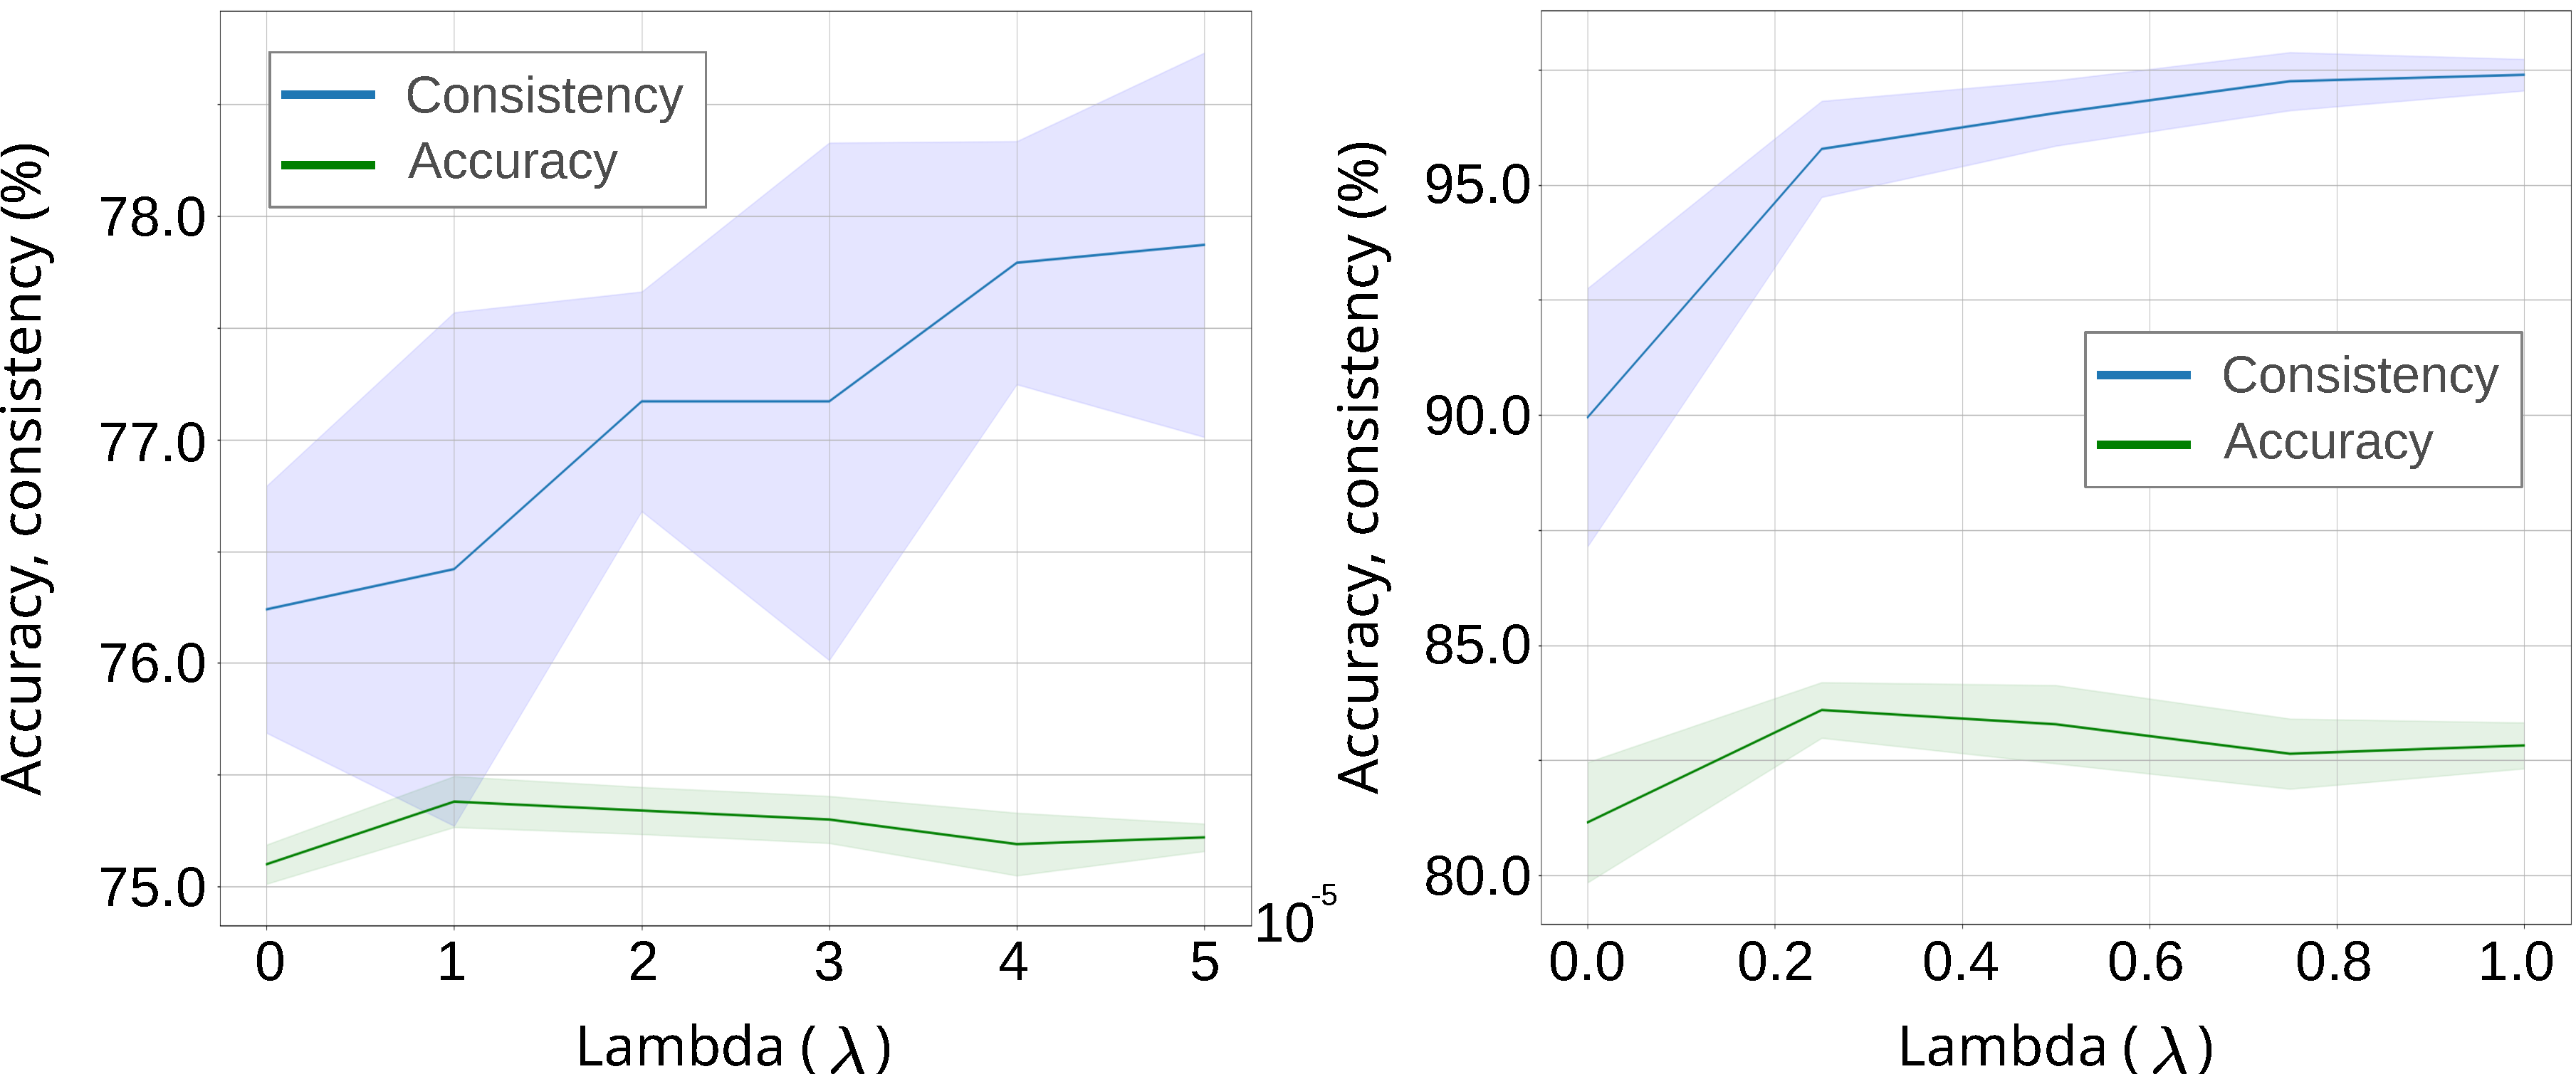
\includegraphics[width=0.8\textwidth]{Figures/Part2_Consist/02_logic/lambda_s.pdf}
\caption{Behavior of the accuracy and consistency as a function of $\lambda$ with 95\% confidence intervals. \textbf{Left:} LXMERT trained on the Introspect dataset (5 models with random seeds for each value of $\lambda$). \textbf{Right:} MVQA trained on the DME dataset (10 models with random seeds for each $\lambda$).}
\label{fig:lambda}
\end{figure}
\subsubsection{Sensitivity of $\bm{\lambda}$}  We now show the sensitivity of our method and its relation to $\lambda$. We evaluate the performance of our method for different values of $\lambda$ to understand the behavior of the performance, both in terms of accuracy and consistency. 

\fig~\ref{fig:lambda} shows the accuracy and consistency of LXMERT and MVQA for different values of $\lambda$. The difference in the ranges of the values is due to the relative magnitude of the loss function terms and depends on the used loss functions (\eg, binary and non-binary cross-entropy) and the ground-truth answer format (\ie, soft scores for LXMERT, as mentioned in Sec.~\ref{subsec:imp_details}). 

In general, we observe very similar behavior for the accuracy, which increases and then slowly decreases as $\lambda$ increases. We sustain that the maximum value the accuracy can reach is established by the number of related pairs that are still inconsistent after training with $\lambda=0$. In other words, the limitations in size impose a limit on how much our method can improve the accuracy. For LXMERT on Introspect, for instance, our model corrected 4,553 (78.9\%) of the 5’771 existing inconsistencies and introduced new inconsistencies by mistakenly altering 1,562 (3.5\%) of the 44,111 consistent samples.

Regarding consistency, we observe a constant increase as $\lambda$ increases. The simultaneous decrease in accuracy as $\lambda$ increases suggests that the relative weight of the consistency loss dominates so that the model no longer focuses on optimizing the cross-entropy. Since it is possible to be consistent without answering correctly, the optimization process results in an increase in consistency at the expense of accuracy for higher values of $\lambda$. However, it is clear from these results that there is a set of $\lambda$ values for which both metrics improve.


 

%\begin{table*}[!t]
%  \centering
%  \begin{tabular}{@{}lccr@{}}
%    \toprule
%    Model & Cons. Method & Acc. & Cons. \\
%    \midrule
%    Base & None & 81.15 & 89.95 \\
%    Base & SQuINT~\cite{selvaraju2020squinting} & 80.58 & 89.39 \\
%    Base & Ours & \textbf{82.85} & \textbf{95.09} \\
%    \bottomrule
%  \end{tabular}
%  \caption{Results on the DME dataset.}
%  \label{tab:cons_logic_results_dme}
%\end{table*}





%\begin{figure}[!t]
%\centering
%\includegraphics[width=0.45\textwidth]{images/dme_plot_consacc_vs_lambda.pdf}
%\caption{Behavior of the accuracy and consistency as a function of the loss term gain $\lambda$ for the DME dataset. 95\% confidence intervals are shown.}
%\label{fig:method}
%\end{figure}


\subsubsection{LI-MOD Performance} We report that the finetuning of \gls{bert} on the subset of annotated relations from Introspect produced $78.67\%$ accuracy in the \gls{nli} task. We analyze the performance of this model for entailment and report an AUC value of 0.86, which indicates good generalization capability considering that only $\approx 2 \%$ of the dataset was annotated with relations. In addition, the overlap in the QA pairs between the train and validation sets of the Introspect dataset is only 1.12\% for binary questions. This shows that our LI-MOD is generalizing to variations in questions and to new combinations of QA pairs. \fig~\ref{fig:roc_dot} shows the \gls{roc} curve for entailment and examples of LI-MOD's predictions. Some of the observed sources of errors in LI-MOD include negations, unusual situation descriptions (\eg, a cat typing a text message), and image-specific references (\eg, ``is \textit{this} animal real?"). 
\begin{figure}
    \centering
    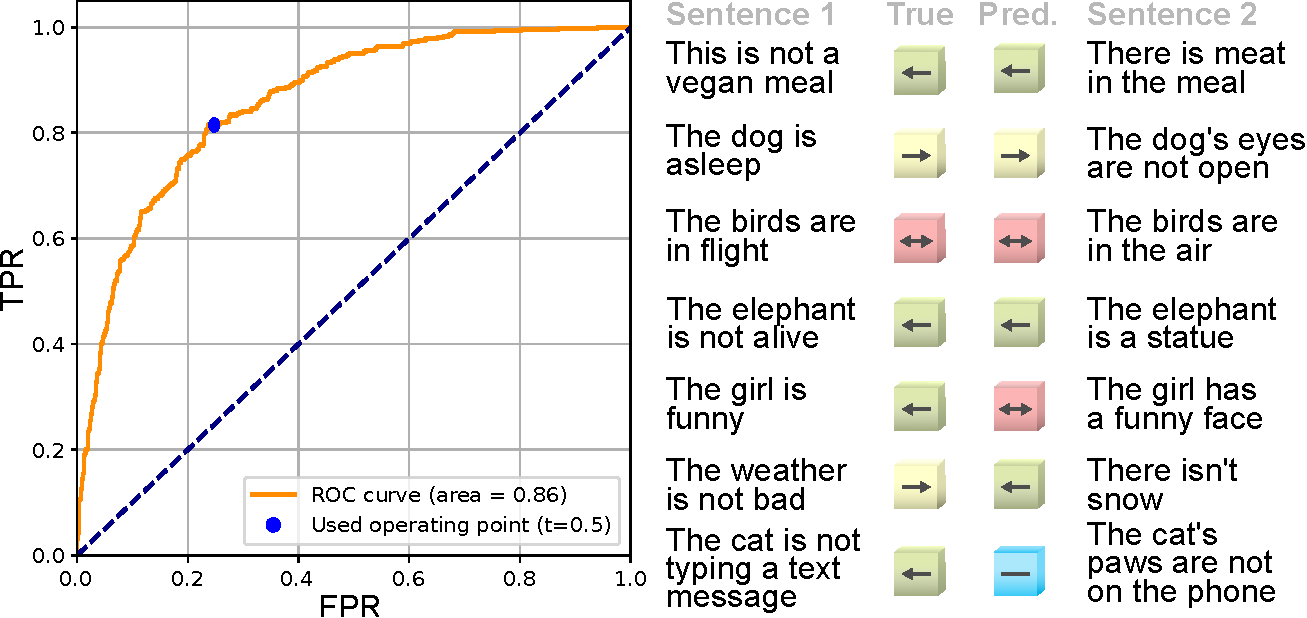
\includegraphics[width=0.8\linewidth]{Figures/Part2_Consist/02_logic/roc_examples_s.pdf}
    \caption{\textbf{Left:} Receiver Operating Characteristic (ROC) for the entailment class of our LI-MOD in validation. \textbf{Right:} Qualitative examples of LI-MOD's predictions.}
    \label{fig:roc_dot}
\end{figure}

%\begin{figure}[!t]
%\centering
%\includegraphics[width=0.4\textwidth]{images/roc.png}
%    \caption{Receiver Operating Characteristic (ROC) for the entailment class of our LI-MOD in validation}
%\label{fig:roc}
%\end{figure}

%\RS{What is the distribution of relations per group in the train and test sets you annotated?} \STM{For train it is $(\leftarrow : 0.595, \leftrightarrow: 0.1725, -: 0.1175, \rightarrow : 0.109, contradictions: 0.006)$. For val it's fairly similar: $(\leftarrow : 0.572, \leftrightarrow: 0.142, -: 0.156, \rightarrow : 0.109)$}

%\begin{figure}[!t]
%\centering
%\includegraphics[width=0.35\textwidth]{images/confusion_matrix_rels.pdf}
%\caption{Confusion matrix for logical implication prediction using our proposed LI-MOD strategy. Note that distribution of labels in both the training used to is given $(\leftarrow : 60\%, \leftrightarrow: 17\%, -: 12\%, \rightarrow : 11\%)$, while the validation set (performance shown here) follows a similar distribution.}
%\label{fig:confusion_matrix}
%\end{figure}
\section{Conclusion}

In this paper, we propose a model-agnostic method to measure and improve consistency in \gls{vqa} by integrating logical implications between pairs of questions in the training process. We also present a method to infer implications between QA pairs using a transformer-based language model. We conduct experiments to validate the generalizability and robustness of our consistency loss against several baselines and across different datasets. Our results show that our method reduces incoherence in responses and improves performance. Future work includes creating a larger dataset with human-annotated relations to use as a general-purpose relations database for \gls{vqa} training.